% Options for packages loaded elsewhere
\PassOptionsToPackage{unicode}{hyperref}
\PassOptionsToPackage{hyphens}{url}
\documentclass[
]{article}
\usepackage{xcolor}
\usepackage[margin=1in]{geometry}
\usepackage{amsmath,amssymb}
\setcounter{secnumdepth}{-\maxdimen} % remove section numbering
\usepackage{iftex}
\ifPDFTeX
  \usepackage[T1]{fontenc}
  \usepackage[utf8]{inputenc}
  \usepackage{textcomp} % provide euro and other symbols
\else % if luatex or xetex
  \usepackage{unicode-math} % this also loads fontspec
  \defaultfontfeatures{Scale=MatchLowercase}
  \defaultfontfeatures[\rmfamily]{Ligatures=TeX,Scale=1}
\fi
\usepackage{lmodern}
\ifPDFTeX\else
  % xetex/luatex font selection
\fi
% Use upquote if available, for straight quotes in verbatim environments
\IfFileExists{upquote.sty}{\usepackage{upquote}}{}
\IfFileExists{microtype.sty}{% use microtype if available
  \usepackage[]{microtype}
  \UseMicrotypeSet[protrusion]{basicmath} % disable protrusion for tt fonts
}{}
\makeatletter
\@ifundefined{KOMAClassName}{% if non-KOMA class
  \IfFileExists{parskip.sty}{%
    \usepackage{parskip}
  }{% else
    \setlength{\parindent}{0pt}
    \setlength{\parskip}{6pt plus 2pt minus 1pt}}
}{% if KOMA class
  \KOMAoptions{parskip=half}}
\makeatother
\usepackage{color}
\usepackage{fancyvrb}
\newcommand{\VerbBar}{|}
\newcommand{\VERB}{\Verb[commandchars=\\\{\}]}
\DefineVerbatimEnvironment{Highlighting}{Verbatim}{commandchars=\\\{\}}
% Add ',fontsize=\small' for more characters per line
\usepackage{framed}
\definecolor{shadecolor}{RGB}{248,248,248}
\newenvironment{Shaded}{\begin{snugshade}}{\end{snugshade}}
\newcommand{\AlertTok}[1]{\textcolor[rgb]{0.94,0.16,0.16}{#1}}
\newcommand{\AnnotationTok}[1]{\textcolor[rgb]{0.56,0.35,0.01}{\textbf{\textit{#1}}}}
\newcommand{\AttributeTok}[1]{\textcolor[rgb]{0.13,0.29,0.53}{#1}}
\newcommand{\BaseNTok}[1]{\textcolor[rgb]{0.00,0.00,0.81}{#1}}
\newcommand{\BuiltInTok}[1]{#1}
\newcommand{\CharTok}[1]{\textcolor[rgb]{0.31,0.60,0.02}{#1}}
\newcommand{\CommentTok}[1]{\textcolor[rgb]{0.56,0.35,0.01}{\textit{#1}}}
\newcommand{\CommentVarTok}[1]{\textcolor[rgb]{0.56,0.35,0.01}{\textbf{\textit{#1}}}}
\newcommand{\ConstantTok}[1]{\textcolor[rgb]{0.56,0.35,0.01}{#1}}
\newcommand{\ControlFlowTok}[1]{\textcolor[rgb]{0.13,0.29,0.53}{\textbf{#1}}}
\newcommand{\DataTypeTok}[1]{\textcolor[rgb]{0.13,0.29,0.53}{#1}}
\newcommand{\DecValTok}[1]{\textcolor[rgb]{0.00,0.00,0.81}{#1}}
\newcommand{\DocumentationTok}[1]{\textcolor[rgb]{0.56,0.35,0.01}{\textbf{\textit{#1}}}}
\newcommand{\ErrorTok}[1]{\textcolor[rgb]{0.64,0.00,0.00}{\textbf{#1}}}
\newcommand{\ExtensionTok}[1]{#1}
\newcommand{\FloatTok}[1]{\textcolor[rgb]{0.00,0.00,0.81}{#1}}
\newcommand{\FunctionTok}[1]{\textcolor[rgb]{0.13,0.29,0.53}{\textbf{#1}}}
\newcommand{\ImportTok}[1]{#1}
\newcommand{\InformationTok}[1]{\textcolor[rgb]{0.56,0.35,0.01}{\textbf{\textit{#1}}}}
\newcommand{\KeywordTok}[1]{\textcolor[rgb]{0.13,0.29,0.53}{\textbf{#1}}}
\newcommand{\NormalTok}[1]{#1}
\newcommand{\OperatorTok}[1]{\textcolor[rgb]{0.81,0.36,0.00}{\textbf{#1}}}
\newcommand{\OtherTok}[1]{\textcolor[rgb]{0.56,0.35,0.01}{#1}}
\newcommand{\PreprocessorTok}[1]{\textcolor[rgb]{0.56,0.35,0.01}{\textit{#1}}}
\newcommand{\RegionMarkerTok}[1]{#1}
\newcommand{\SpecialCharTok}[1]{\textcolor[rgb]{0.81,0.36,0.00}{\textbf{#1}}}
\newcommand{\SpecialStringTok}[1]{\textcolor[rgb]{0.31,0.60,0.02}{#1}}
\newcommand{\StringTok}[1]{\textcolor[rgb]{0.31,0.60,0.02}{#1}}
\newcommand{\VariableTok}[1]{\textcolor[rgb]{0.00,0.00,0.00}{#1}}
\newcommand{\VerbatimStringTok}[1]{\textcolor[rgb]{0.31,0.60,0.02}{#1}}
\newcommand{\WarningTok}[1]{\textcolor[rgb]{0.56,0.35,0.01}{\textbf{\textit{#1}}}}
\usepackage{longtable,booktabs,array}
\usepackage{calc} % for calculating minipage widths
% Correct order of tables after \paragraph or \subparagraph
\usepackage{etoolbox}
\makeatletter
\patchcmd\longtable{\par}{\if@noskipsec\mbox{}\fi\par}{}{}
\makeatother
% Allow footnotes in longtable head/foot
\IfFileExists{footnotehyper.sty}{\usepackage{footnotehyper}}{\usepackage{footnote}}
\makesavenoteenv{longtable}
\usepackage{graphicx}
\makeatletter
\newsavebox\pandoc@box
\newcommand*\pandocbounded[1]{% scales image to fit in text height/width
  \sbox\pandoc@box{#1}%
  \Gscale@div\@tempa{\textheight}{\dimexpr\ht\pandoc@box+\dp\pandoc@box\relax}%
  \Gscale@div\@tempb{\linewidth}{\wd\pandoc@box}%
  \ifdim\@tempb\p@<\@tempa\p@\let\@tempa\@tempb\fi% select the smaller of both
  \ifdim\@tempa\p@<\p@\scalebox{\@tempa}{\usebox\pandoc@box}%
  \else\usebox{\pandoc@box}%
  \fi%
}
% Set default figure placement to htbp
\def\fps@figure{htbp}
\makeatother
\setlength{\emergencystretch}{3em} % prevent overfull lines
\providecommand{\tightlist}{%
  \setlength{\itemsep}{0pt}\setlength{\parskip}{0pt}}
\usepackage{bookmark}
\IfFileExists{xurl.sty}{\usepackage{xurl}}{} % add URL line breaks if available
\urlstyle{same}
\hypersetup{
  pdftitle={Dashboards for Clicker Data},
  pdfauthor={Sydney Chin (scc273), Younghyun Jung (yj582), Arianna Hsu (ach282), Ivy Liu (il328), Amy Oduor (aao73), Sheki Okwayo(lso24)},
  hidelinks,
  pdfcreator={LaTeX via pandoc}}

\title{Dashboards for Clicker Data}
\usepackage{etoolbox}
\makeatletter
\providecommand{\subtitle}[1]{% add subtitle to \maketitle
  \apptocmd{\@title}{\par {\large #1 \par}}{}{}
}
\makeatother
\subtitle{INFO 4100 Learning Analytics}
\author{Sydney Chin (scc273), Younghyun Jung (yj582), Arianna Hsu
(ach282), Ivy Liu (il328), Amy Oduor (aao73), Sheki Okwayo(lso24)}
\date{}

\begin{document}
\maketitle

This project is about developing a learning analytics dashboard based on
clicker data. You will work as a team to learn how to make a dashboard
using R Shiny (official page with several tutorials:
\url{https://shiny.rstudio.com/tutorial/}).

\textbf{Learning Objectives}

\begin{enumerate}
\def\labelenumi{\arabic{enumi}.}
\tightlist
\item
  Understand the structure of clicker data
\item
  Create multiple different visualizations
\item
  Design and implement an instructor and student dashboard
\item
  Critically evaluate your own dashboard design
\end{enumerate}

You are given aggregated clicker records for a CS course taught at
Cornell. There are two datasets: the experience dataset and the quiz
dataset.

\textbf{Scenario}

You are approached by a college instructor who uses iClickers in her CS
class on Business Intelligence. She would like to gain insights about
her students and how they are engaging/performing in order to better
help them in class. She would also like to better support students by
giving them feedback at scale about where they stand and perhaps how
they compare to others in the class.

You offer to build a prototype of a dashboard using her clicker data:
this is a dashboard for the instructor which offers an overview of the
class characteristics, engagement, and performance; and it is a
dashboard for students which offers a specific student an overview of
their engagement and performance (and how it compares to others).

\textbf{Data}

The \textbf{experience dataset} contains one record per student who
completed the CS course between 2016-2018. There are two sources to this
dataset: Faculty Center and a Skills Survey (administered via the
Blackboard LMS) where students self reported their skill level for
various skills the first week of class. This data has been
de-identified. Name, netid, emplid, major have all been removed and
replaced with a unique numeric identifier. Note that not all students
completed the skills survey, they will have null values for the survey
result fields.

\begin{longtable}[]{@{}
  >{\raggedright\arraybackslash}p{(\linewidth - 4\tabcolsep) * \real{0.1376}}
  >{\raggedright\arraybackslash}p{(\linewidth - 4\tabcolsep) * \real{0.1693}}
  >{\raggedright\arraybackslash}p{(\linewidth - 4\tabcolsep) * \real{0.6931}}@{}}
\toprule\noalign{}
\begin{minipage}[b]{\linewidth}\raggedright
Attribute Name
\end{minipage} & \begin{minipage}[b]{\linewidth}\raggedright
Data Type
\end{minipage} & \begin{minipage}[b]{\linewidth}\raggedright
Definition
\end{minipage} \\
\midrule\noalign{}
\endhead
\bottomrule\noalign{}
\endlastfoot
student\_key & numeric Unique key & Assigned as part of
de-identification process. Uniquely identifies student records for this
data set only. \\
year & numeric & Four digit year student was enrolled in BI Class. \\
prog & character Values (GRAD, UGRAD) & Indicates whether the student
was a graduate or undergraduate student when they were enrolled in BI
course. \\
database\_score & numeric (0-5) & Self reported experience level with
database technology prior to taking course. 0= no experience, 5=
expertise \\
sql\_score & numeric (0-5) & Self reported experience level with SQL
prior to taking course. 0= no experience, 5=expertise \\
programing\_score & numeric (0-5) & Self reported experience level with
Any Programing language prior to taking course. 0=no experience,
5=expertise \\
stored\_proc\_score & numeric (0-5) & Self reported experience level
with stored procedure languages prior to taking course. 0=no experience,
5=expertise \\
etl\_score & numeric (0-5) & Self reported experience level with Extract
Transform Load (ETL) development prior to taking course. 0=no
experience, 5=expertise \\
data\_vis\_score & numeric (0-5) & Self reported experience level using
data visualization tools prior to taking course. 0=no experience,
5=expertise \\
requirement\_gather\_score & numeric (0-5) & Self reported experience
level gathering customer requirements prior to taking course. 0=no
experience, 5=expertise \\
skill\_survey\_score & numeric & Sum of the self reported skill level
scores. \\
\end{longtable}

The \textbf{quiz dataset} contains one record per student per class
session held where iClickers were used. Sources used in the creation of
this data set include: iClicker session xml files, Blackboard gradebook
(for quiz scores), and the Blackboard class schedule (used to map
iClicker session to related quiz scores). Note that in some cases there
are multiple iClicker sessions / lectures associated with a single quiz.
This dataset may be joined to the experience dataset by the student\_key
field.

\begin{longtable}[]{@{}
  >{\raggedright\arraybackslash}p{(\linewidth - 4\tabcolsep) * \real{0.0833}}
  >{\raggedright\arraybackslash}p{(\linewidth - 4\tabcolsep) * \real{0.0500}}
  >{\raggedright\arraybackslash}p{(\linewidth - 4\tabcolsep) * \real{0.8667}}@{}}
\toprule\noalign{}
\begin{minipage}[b]{\linewidth}\raggedright
Attribute Name
\end{minipage} & \begin{minipage}[b]{\linewidth}\raggedright
Data Type
\end{minipage} & \begin{minipage}[b]{\linewidth}\raggedright
Definition
\end{minipage} \\
\midrule\noalign{}
\endhead
\bottomrule\noalign{}
\endlastfoot
Acad\_date\_key & numeric & Date key in the form of YYYYMMDD indicating
the date the class session was held. \\
student\_key & numeric & Unique identifier for students who took BI
class 2016-2018. This key is the primary key for the experience\_data
file. \\
year & numeric & Four digit year class session was held. \\
session\_number & numeric & Identifies the session number for a
particular semester. Session number is assigned by iClicker. \\
quiz\_number & numeric & There are 10 quizzes throughout the BI course.
This attribute indicates which quiz is associated with the iClicker
session(s). \\
attended & numeric (0,1) & Binary indicating whether the student
attended that particular class session / lecture. 0=no, 1=yes. \\
total\_possible\_clicker & numeric & The total number of iClicker
questions asked that session. \\
total\_completed\_clicker & numeric & The number of iClicker questions
answered by student that session. \\
completed\_q\_clicker & numeric & The number of completed Quiz iClicker
questions \\
correct\_q\_clicker & numeric & How many correct Quiz answers by student
that session. \\
completed\_t\_clicker & number & How many Temperature questions answered
by student that session. Temperature questions are 0-5, 0= bad, 5=great.
There is no correct answer to Temperature questions, they are used to
guage how students are feeling about a particular subject, assignment,
etc. \\
avg\_t\_clicker & number & The average temperature answer by student for
that session. An average of 1 or 2 would be generally negative, while 4
or 5 would be generally positive responses. \\
quiz\_score & numeric & Quiz score out of 20 points possible. \\
\end{longtable}

\section{Part 1: Planning / Sketching}\label{part-1-planning-sketching}

Go through the planning / sketching process described in the reading
about dashboards. While some dashboards are certainly better than
others, there is not one correct solution here. However, spending enough
time to make a concrete plan is essential for the success of your
project. Everything you do to make the dashboards will be easier if you
have a clear plan, especially because you will be splitting up the work
and everyone needs to know what they should work on.

\textbf{Question 1:} You will make a student dashboard and a teacher
dashboard. Carefully consider the implications of this for design and
content. To plan, answer the following prompts once for the student
dashboard and then for the teacher dashboard. The more concrete you are
here the easier it will be later. Focus on the concrete ideas that you
will implement in the next steps. You can iterate on this step and
modify your responses as your ideas for the dashboard become clearer.
You should explore the dataset in R for 5-10 minutes to get a good sense
of what the dataset has to offer.

\emph{Planning for the student dashboard}

\begin{itemize}
\tightlist
\item
  For whom? Who will use it and what is their background?

  \begin{itemize}
  \tightlist
  \item
    Students have a mix of backgrounds including both undergrad and
    graduate students. They will use this dashboard to know their
    standing compared to other students in the class.
  \end{itemize}
\item
  Why? What is the goal? What questions to answer?

  \begin{itemize}
  \tightlist
  \item
    The student's goal is to be able to assess their understanding of
    the content so they know when to ask for help. Additionally, it is
    helpful to know their attendance rate in order to maximize their
    participation grade.
  \end{itemize}
\item
  What? What data to show and what is its structure?

  \begin{itemize}
  \tightlist
  \item
    {[}add your answer here{]}
  \item
    {[}add your answer here{]}
  \end{itemize}
\item
  How? How will visualizations support the goal?

  \begin{itemize}
  \tightlist
  \item
    {[}add your answer here{]}
  \item
    {[}add your answer here{]}
  \end{itemize}
\end{itemize}

\emph{Planning for the teacher dashboard}

\begin{itemize}
\tightlist
\item
  For whom? Who will use it and what is their background?

  \begin{itemize}
  \tightlist
  \item
    The instructor is teaching a large class, so it is hard to be able
    to gauge how every student is doing. The teacher would like more
    support in pinpointing which students need additional interventions.
  \end{itemize}
\item
  Why? What is the goal? What questions to answer?

  \begin{itemize}
  \tightlist
  \item
    The instructor would like to know which sessions students were able
    to understand well and which sessions were confusing. Also, it is
    important to know which students are struggling to understand the
    course content.
  \end{itemize}
\item
  What? What data to show and what is its structure?

  \begin{itemize}
  \tightlist
  \item
    {[}add your answer here{]}
  \item
    {[}add your answer here{]}
  \end{itemize}
\item
  How? How will visualizations support the goal?

  \begin{itemize}
  \tightlist
  \item
    The skills gap visualization will help the instructor know which
    students have incorrectly assessed their skills (had high survey
    scores but low quiz scores) and which students are struggling due to
    their lack of prior knowledge (had low survey scores and currently
    have low quiz scores).
  \end{itemize}
\end{itemize}

\textbf{Question 2:} Based on your plan above, make a sketch of what the
dashboard would look like. See this week's readings for examples. Be
detailed about what kinds of data points and visualizations you want to
see in different parts of the page. Consider the user experience and how
you should position more general information compared to more specific
information, and where you may need some additional explanation to help
the viewer understand a graphic, for example. In your sketch, it is
useful to give labels to different objects, because in the steps below
you can split up work between team members and the labels will help you
connect the UI with the data objects. Show your sketches in section to
get feedback from the teaching team.

Each dashboard should contain at least 4 data visualizations. You may
include any additional summary statistics (e.g.~key percentages or
tables).

\section{Part 2: Dashboard Wire-frame
Implementation}\label{part-2-dashboard-wire-frame-implementation}

This is where you generate the dashboard layout. You are given a very
basic wire frame example for the dashboard below. For more information
on how R Shiny Dashboards work, look at
\url{https://rstudio.github.io/shinydashboard/get_started.html} and
\url{https://rstudio.github.io/shinydashboard/structure.html}. You can
add different types of content into a \texttt{fuidRow()}. In the starter
code, there are 2 rows of content: the first has two little info boxes;
the second has two larger viz boxes. You can add more rows and change
what is in them as you wish. Follow the naming convention,
e.g.~\texttt{inst.info1} is the first info box for instructors.

Your team can split up the tasks. Some work on creating the UI (this
part), while others work on pre-processing the data and creating the
statistics and visualizations that will populate the UI (next part).

\textbf{Question 3:} Create the layout for the dashboard tabs. You can
have as many ``tabs'' as you like. Each tab is the content displayed
when the user clicks on one of the menu items (so it is the page
content). Here you are just specifying the wire frame i.e.~\textbf{what
goes where on the pages}, not what goes into it.

\begin{Shaded}
\begin{Highlighting}[]
\DocumentationTok{\#\#\#\#\#\#\#\#\#\#\#\#\#\#\#\#\#\#\#\#\#\#\#\#\#\#\#\#\#\#\#\#\#\#\#\#\#\#\#}
\DocumentationTok{\#\#\#\#\#\#\# }\RegionMarkerTok{BEGIN}\DocumentationTok{ INPUT: Question 3 \#\#\#\#\#\#\#}
\DocumentationTok{\#\#\#\#\#\#\#\#\#\#\#\#\#\#\#\#\#\#\#\#\#\#\#\#\#\#\#\#\#\#\#\#\#\#\#\#\#\#\#}

\CommentTok{\# =====================}
\CommentTok{\# INSTRUCTOR DASHBOARD}
\CommentTok{\# =====================}
\NormalTok{instructor\_dash }\OtherTok{\textless{}{-}} \FunctionTok{tabItem}\NormalTok{(}
  \AttributeTok{tabName =} \StringTok{"instructor"}\NormalTok{,}
  \FunctionTok{h2}\NormalTok{(}\StringTok{"Instructor Dashboard"}\NormalTok{),}
  
  \FunctionTok{fluidRow}\NormalTok{(}
    \FunctionTok{box}\NormalTok{(}
      \AttributeTok{title =} \StringTok{"Instructor Filters"}\NormalTok{, }\AttributeTok{width =} \DecValTok{12}\NormalTok{, }\AttributeTok{status =} \StringTok{"primary"}\NormalTok{,}
      \FunctionTok{column}\NormalTok{(}\DecValTok{4}\NormalTok{, }\FunctionTok{selectInput}\NormalTok{(}\StringTok{"inst.year"}\NormalTok{, }\StringTok{"Select Year"}\NormalTok{, }\AttributeTok{choices =} \FunctionTok{c}\NormalTok{(}\StringTok{"All"}\NormalTok{), }\AttributeTok{selected =} \StringTok{"All"}\NormalTok{)),}
      \FunctionTok{column}\NormalTok{(}\DecValTok{4}\NormalTok{, }\FunctionTok{sliderInput}\NormalTok{(}\StringTok{"inst.attend\_cutoff"}\NormalTok{, }\StringTok{"Risk Attendance Cutoff (\%)"}\NormalTok{, }\AttributeTok{min =} \DecValTok{40}\NormalTok{, }\AttributeTok{max =} \DecValTok{95}\NormalTok{, }\AttributeTok{value =} \DecValTok{75}\NormalTok{, }\AttributeTok{step =} \DecValTok{5}\NormalTok{)),}
      \FunctionTok{column}\NormalTok{(}\DecValTok{4}\NormalTok{, }\FunctionTok{sliderInput}\NormalTok{(}\StringTok{"inst.quiz\_cutoff"}\NormalTok{, }\StringTok{"Risk Avg Quiz Score Cutoff"}\NormalTok{, }\AttributeTok{min =} \DecValTok{8}\NormalTok{, }\AttributeTok{max =} \DecValTok{18}\NormalTok{, }\AttributeTok{value =} \DecValTok{14}\NormalTok{, }\AttributeTok{step =} \DecValTok{1}\NormalTok{))}
\NormalTok{    )}
\NormalTok{  ),}
  
  \CommentTok{\# KPI Boxes}
  \FunctionTok{fluidRow}\NormalTok{(}
    \FunctionTok{infoBoxOutput}\NormalTok{(}\StringTok{"inst.total\_students"}\NormalTok{, }\AttributeTok{width =} \DecValTok{3}\NormalTok{),}
    \FunctionTok{infoBoxOutput}\NormalTok{(}\StringTok{"inst.avg\_attendance"}\NormalTok{, }\AttributeTok{width =} \DecValTok{3}\NormalTok{),}
    \FunctionTok{infoBoxOutput}\NormalTok{(}\StringTok{"inst.avg\_score"}\NormalTok{, }\AttributeTok{width =} \DecValTok{3}\NormalTok{),}
    \FunctionTok{infoBoxOutput}\NormalTok{(}\StringTok{"inst.avg\_sentiment"}\NormalTok{, }\AttributeTok{width =} \DecValTok{3}\NormalTok{)}
\NormalTok{  ),}
  
  \CommentTok{\# Charts}
  \FunctionTok{fluidRow}\NormalTok{(}
    \FunctionTok{box}\NormalTok{(}
      \AttributeTok{title =} \StringTok{"Quiz Score Trend"}\NormalTok{, }\AttributeTok{width =} \DecValTok{6}\NormalTok{,}
      \FunctionTok{plotOutput}\NormalTok{(}\StringTok{"inst.quiz\_trend"}\NormalTok{, }\AttributeTok{height =} \DecValTok{250}\NormalTok{)}
\NormalTok{    ),}
    \FunctionTok{box}\NormalTok{(}
      \AttributeTok{title =} \StringTok{"Skill to Performance Gap"}\NormalTok{, }\AttributeTok{width =} \DecValTok{6}\NormalTok{,}
      \FunctionTok{plotOutput}\NormalTok{(}\StringTok{"inst.skill\_gap\_plot"}\NormalTok{, }\AttributeTok{height =} \DecValTok{250}\NormalTok{)}
\NormalTok{    )}
\NormalTok{  ),}
  
  \CommentTok{\# At{-}Risk Analytics}
  \FunctionTok{fluidRow}\NormalTok{(}
    \FunctionTok{box}\NormalTok{(}
      \AttributeTok{title =} \StringTok{"Student Intervention Map"}\NormalTok{, }\AttributeTok{width =} \DecValTok{6}\NormalTok{,}
      \FunctionTok{plotlyOutput}\NormalTok{(}\StringTok{"inst.risk.map"}\NormalTok{, }\AttributeTok{height =} \DecValTok{300}\NormalTok{)}
\NormalTok{    ),}
    \FunctionTok{box}\NormalTok{(}
      \AttributeTok{title =} \StringTok{"At{-}Risk Students List"}\NormalTok{, }\AttributeTok{width =} \DecValTok{6}\NormalTok{,}
      \FunctionTok{div}\NormalTok{(}\AttributeTok{style =} \StringTok{"height: 300px; overflow{-}y: auto;"}\NormalTok{,}
          \FunctionTok{tableOutput}\NormalTok{(}\StringTok{"inst.risk.table"}\NormalTok{)}
\NormalTok{      )}
\NormalTok{    )}
\NormalTok{  )}
\NormalTok{)}

\CommentTok{\# =====================}
\CommentTok{\# STUDENT DASHBOARD}
\CommentTok{\# =====================}
\NormalTok{student\_dash }\OtherTok{\textless{}{-}} \FunctionTok{tabItem}\NormalTok{(}
  \AttributeTok{tabName =} \StringTok{"student"}\NormalTok{,}
  \FunctionTok{h2}\NormalTok{(}\StringTok{"Student Dashboard"}\NormalTok{),}
  \FunctionTok{fluidRow}\NormalTok{(}
    \FunctionTok{infoBoxOutput}\NormalTok{(}\StringTok{"stu.attendance"}\NormalTok{),}
    \FunctionTok{infoBoxOutput}\NormalTok{(}\StringTok{"stu.avg\_score"}\NormalTok{),}
    \FunctionTok{infoBoxOutput}\NormalTok{(}\StringTok{"stu.clicker\_acc"}\NormalTok{),}
    \FunctionTok{infoBoxOutput}\NormalTok{(}\StringTok{"stu.sentiment"}\NormalTok{)}
\NormalTok{  ),}
  \FunctionTok{fluidRow}\NormalTok{(}
    \FunctionTok{box}\NormalTok{(}
      \AttributeTok{title =} \StringTok{"My Quiz Scores vs Class Average"}\NormalTok{, }\AttributeTok{width =} \DecValTok{6}\NormalTok{,}
      \FunctionTok{plotOutput}\NormalTok{(}\StringTok{"stu.quiz\_compare"}\NormalTok{, }\AttributeTok{height =} \DecValTok{250}\NormalTok{)}
\NormalTok{    ),}
    \FunctionTok{box}\NormalTok{(}
      \AttributeTok{title =} \StringTok{"My Attendance per Session"}\NormalTok{, }\AttributeTok{width =} \DecValTok{6}\NormalTok{,}
      \FunctionTok{plotOutput}\NormalTok{(}\StringTok{"stu.attendance\_plot"}\NormalTok{, }\AttributeTok{height =} \DecValTok{250}\NormalTok{)}
\NormalTok{    )}
\NormalTok{  ),}
  \FunctionTok{fluidRow}\NormalTok{(}
    \FunctionTok{box}\NormalTok{(}
      \AttributeTok{title =} \StringTok{"My sentiment vs class average"}\NormalTok{,}
      \AttributeTok{width =} \DecValTok{6}\NormalTok{,}
      \FunctionTok{plotOutput}\NormalTok{(}\StringTok{"stu.sentiment\_plot"}\NormalTok{, }\AttributeTok{height =} \DecValTok{250}\NormalTok{)}
\NormalTok{    ),}
    \FunctionTok{box}\NormalTok{(}
      \AttributeTok{title =} \StringTok{"My Skill Profile vs Class Average"}\NormalTok{,}
      \AttributeTok{width =} \DecValTok{6}\NormalTok{,}
      \FunctionTok{plotOutput}\NormalTok{(}\StringTok{"stu.plot4"}\NormalTok{, }\AttributeTok{height =} \DecValTok{250}\NormalTok{)}
\NormalTok{    )}
\NormalTok{  )}
\NormalTok{)}

\DocumentationTok{\#\#\#\#\#\#\#\#\#\#\#\#\#\#\#\#\#\#\#\#\#\#\#\#\#\#\#\#\#\#\#\#\#\#\#\#\#\#\#}
\DocumentationTok{\#\#\#\#\#\#\#\#\#\#\#\#\#\#\#\#\#\#\#\#\#\#\#\#\#\#\#\#\#\#\#\#\#\#\#\#\#\#\#}
\end{Highlighting}
\end{Shaded}

\section{Part 3: Data Pre-processing}\label{part-3-data-pre-processing}

Get the data ready for use in the dashboard. Before the next stage, you
want to have the data ready in the right format for simple computations
and plotting. To do this effectively, you need to know by now what you
want to display in each dashboard. However, this is also an iterative
process. Once you have completed a first iteration of the design, you
can come back to this step and add further pre-processing for more
visualizations you like to add. This step is also an opportunity to
better understand the structure of the datasets.

The instructor dashboard should show information for all students. The
student dashboard is typically focused on an individual student. You can
either pick a student (at random or intentionally) and use them as the
``reference student'' for the student dashboard. Or, a bit more
ambitious but also more rewarding to try out, you can create an
interactive dashboard in which you select the student and then the
dashboard updates to show the information for that student. I would
recommend you start with the simpler version and get that to work before
you try to make it dynamic.

Use the space below to be ready for your information visualizations in
the dashboards.

\begin{Shaded}
\begin{Highlighting}[]
\DocumentationTok{\#\#\#\#\#\#\#\#\#\#\#\#\#\#\#\#\#\#\#\#\#\#\#\#\#\#\#\#\#\#\#\#\#\#\#\#\#\#\#}
\DocumentationTok{\#\#\#\#\#\#\# }\RegionMarkerTok{BEGIN}\DocumentationTok{ INPUT             \#\#\#\#\#\#\#}
\DocumentationTok{\#\#\#\#\#\#\#\#\#\#\#\#\#\#\#\#\#\#\#\#\#\#\#\#\#\#\#\#\#\#\#\#\#\#\#\#\#\#\#}

\DocumentationTok{\#\#\#\#\#\#\#\#\#\#\#\#\#\#\#\#\#\#\#\#\#\#\#\#\#\#\#\#\#\#\#\#\#\#\#\#\#\#}
\DocumentationTok{\#\#\#\#\#\#\# QUIZ SCORE DATA        \#\#\#\#\#\#\#}
\DocumentationTok{\#\#\#\#\#\#\#\#\#\#\#\#\#\#\#\#\#\#\#\#\#\#\#\#\#\#\#\#\#\#\#\#\#\#\#\#\#\#}

\NormalTok{quiz\_clean }\OtherTok{\textless{}{-}}\NormalTok{ quiz }\SpecialCharTok{\%\textgreater{}\%}
  \FunctionTok{mutate}\NormalTok{(}
    \AttributeTok{clicker\_completion\_rate =} \FunctionTok{if\_else}\NormalTok{(}
\NormalTok{      TOTAL\_POSSIBLE\_CLICKER }\SpecialCharTok{\textgreater{}} \DecValTok{0}\NormalTok{,}
\NormalTok{      TOTAL\_COMPLETED\_CLICKER }\SpecialCharTok{/}\NormalTok{ TOTAL\_POSSIBLE\_CLICKER,}
      \ConstantTok{NA\_real\_}
\NormalTok{    )}
\NormalTok{  )}

\NormalTok{experience\_clean }\OtherTok{\textless{}{-}}\NormalTok{ experience}

\NormalTok{inst\_year\_choices }\OtherTok{\textless{}{-}} \FunctionTok{c}\NormalTok{(}\StringTok{"All"}\NormalTok{, }\FunctionTok{sort}\NormalTok{(}\FunctionTok{unique}\NormalTok{(quiz\_clean}\SpecialCharTok{$}\NormalTok{YEAR)))}
\NormalTok{student\_choices }\OtherTok{\textless{}{-}} \FunctionTok{sort}\NormalTok{(}\FunctionTok{unique}\NormalTok{(quiz\_clean}\SpecialCharTok{$}\NormalTok{STUDENT\_KEY))}
\NormalTok{reference\_student\_key }\OtherTok{\textless{}{-}}\NormalTok{ student\_choices[}\DecValTok{1}\NormalTok{]}
\NormalTok{all\_sessions }\OtherTok{\textless{}{-}} \FunctionTok{sort}\NormalTok{(}\FunctionTok{unique}\NormalTok{(quiz\_clean}\SpecialCharTok{$}\NormalTok{SESSION\_NUMBER))}

\NormalTok{skill\_cols }\OtherTok{\textless{}{-}} \FunctionTok{c}\NormalTok{(}
  \StringTok{"DATABASE\_SCORE"}\NormalTok{, }\StringTok{"SQL\_SCORE"}\NormalTok{, }\StringTok{"PROGRAMING\_SCORE"}\NormalTok{,}
  \StringTok{"STORED\_PROC\_SCORE"}\NormalTok{, }\StringTok{"ETL\_SCORE"}\NormalTok{, }\StringTok{"DATA\_VIS\_SCORE"}\NormalTok{,}
  \StringTok{"REQUIREMENT\_GATHER\_SCORE"}
\NormalTok{)}

\NormalTok{class\_avg }\OtherTok{\textless{}{-}}\NormalTok{ experience\_clean }\SpecialCharTok{\%\textgreater{}\%}
  \FunctionTok{summarise}\NormalTok{(}\FunctionTok{across}\NormalTok{(}\FunctionTok{all\_of}\NormalTok{(skill\_cols), mean, }\AttributeTok{na.rm =} \ConstantTok{TRUE}\NormalTok{))}
\end{Highlighting}
\end{Shaded}

\begin{verbatim}
## Warning: There was 1 warning in `summarise()`.
## i In argument: `across(all_of(skill_cols), mean, na.rm = TRUE)`.
## Caused by warning:
## ! The `...` argument of `across()` is deprecated as of dplyr 1.1.0.
## Supply arguments directly to `.fns` through an anonymous function instead.
## 
##   # Previously
##   across(a:b, mean, na.rm = TRUE)
## 
##   # Now
##   across(a:b, \(x) mean(x, na.rm = TRUE))
\end{verbatim}

\begin{Shaded}
\begin{Highlighting}[]
\DocumentationTok{\#\#\#\#\#\#\#\#\#\#\#\#\#\#\#\#\#\#\#\#\#\#\#\#\#\#\#\#\#\#\#\#\#\#\#\#\#\#\#}
\DocumentationTok{\#\#\#\#\#\#\#\#\#\#\#\#\#\#\#\#\#\#\#\#\#\#\#\#\#\#\#\#\#\#\#\#\#\#\#\#\#\#\#}
\end{Highlighting}
\end{Shaded}

\section{Part 4: Prepare All Data
Visualizations}\label{part-4-prepare-all-data-visualizations}

This is where you create the content for the wire frames you created
above. Again, you can refer to the examples and documentation in
\url{https://rstudio.github.io/shinydashboard/get_started.html} and
\url{https://rstudio.github.io/shinydashboard/structure.html} for
guidance. You can also find many examples online just by searching with
Google.

\textbf{Question 4:} For each of the pieces of content you planned for
in the wire frames above, generate the relevant content. You need to
assign them all to the \texttt{output} variable by referencing the name
of the wire frame element you chose above like this
\texttt{output\$name.of.element}.

\begin{Shaded}
\begin{Highlighting}[]
\NormalTok{server }\OtherTok{\textless{}{-}} \ControlFlowTok{function}\NormalTok{(input, output, session) \{}
  \DocumentationTok{\#\#\#\#\#\#\#\#\#\#\#\#\#\#\#\#\#\#\#\#\#\#\#\#\#\#\#\#\#\#\#\#\#\#\#\#\#\#\#}
  \DocumentationTok{\#\#\#\#\#\#\# }\RegionMarkerTok{BEGIN}\DocumentationTok{ INPUT: Question 4 \#\#\#\#\#\#\#}
  \DocumentationTok{\#\#\#\#\#\#\#\#\#\#\#\#\#\#\#\#\#\#\#\#\#\#\#\#\#\#\#\#\#\#\#\#\#\#\#\#\#\#\#}
  
  \FunctionTok{updateSelectInput}\NormalTok{(session, }\StringTok{"inst.year"}\NormalTok{, }\AttributeTok{choices =}\NormalTok{ inst\_year\_choices, }\AttributeTok{selected =} \StringTok{"All"}\NormalTok{)}
  \FunctionTok{updateSelectInput}\NormalTok{(session, }\StringTok{"stud.key"}\NormalTok{, }\AttributeTok{choices =}\NormalTok{ student\_choices, }\AttributeTok{selected =}\NormalTok{ reference\_student\_key)}

\NormalTok{  instructor\_filtered }\OtherTok{\textless{}{-}} \FunctionTok{reactive}\NormalTok{(\{}
    \FunctionTok{req}\NormalTok{(input}\SpecialCharTok{$}\NormalTok{inst.year)}
    \ControlFlowTok{if}\NormalTok{ (input}\SpecialCharTok{$}\NormalTok{inst.year }\SpecialCharTok{==} \StringTok{"All"}\NormalTok{) \{}
\NormalTok{      quiz\_clean}
\NormalTok{    \} }\ControlFlowTok{else}\NormalTok{ \{}
\NormalTok{      quiz\_clean }\SpecialCharTok{\%\textgreater{}\%} \FunctionTok{filter}\NormalTok{(YEAR }\SpecialCharTok{==} \FunctionTok{as.numeric}\NormalTok{(input}\SpecialCharTok{$}\NormalTok{inst.year))}
\NormalTok{    \}}
\NormalTok{  \})}

\NormalTok{  instructor\_student\_rollup }\OtherTok{\textless{}{-}} \FunctionTok{reactive}\NormalTok{(\{}
    \FunctionTok{instructor\_filtered}\NormalTok{() }\SpecialCharTok{\%\textgreater{}\%}
      \FunctionTok{group\_by}\NormalTok{(STUDENT\_KEY) }\SpecialCharTok{\%\textgreater{}\%}
      \FunctionTok{summarise}\NormalTok{(}
        \AttributeTok{attendance\_rate =} \FunctionTok{mean}\NormalTok{(ATTENDED, }\AttributeTok{na.rm =} \ConstantTok{TRUE}\NormalTok{),}
        \AttributeTok{avg\_quiz\_score =} \FunctionTok{mean}\NormalTok{(QUIZ\_SCORE, }\AttributeTok{na.rm =} \ConstantTok{TRUE}\NormalTok{),}
        \AttributeTok{sessions =} \FunctionTok{n}\NormalTok{(),}
        \AttributeTok{.groups =} \StringTok{"drop"}
\NormalTok{      )}
\NormalTok{  \})}

\NormalTok{  at\_risk\_filtered }\OtherTok{\textless{}{-}} \FunctionTok{reactive}\NormalTok{(\{}
    \FunctionTok{req}\NormalTok{(input}\SpecialCharTok{$}\NormalTok{inst.attend\_cutoff, input}\SpecialCharTok{$}\NormalTok{inst.quiz\_cutoff)}
    \FunctionTok{instructor\_student\_rollup}\NormalTok{() }\SpecialCharTok{\%\textgreater{}\%}
      \FunctionTok{mutate}\NormalTok{(}
        \AttributeTok{risk\_group =} \FunctionTok{case\_when}\NormalTok{(}
\NormalTok{          attendance\_rate }\SpecialCharTok{\textless{}}\NormalTok{ (input}\SpecialCharTok{$}\NormalTok{inst.attend\_cutoff }\SpecialCharTok{/} \DecValTok{100}\NormalTok{) }\SpecialCharTok{\&}\NormalTok{ avg\_quiz\_score }\SpecialCharTok{\textless{}}\NormalTok{ input}\SpecialCharTok{$}\NormalTok{inst.quiz\_cutoff }\SpecialCharTok{\textasciitilde{}} \StringTok{"Low Attendance \& Score"}\NormalTok{,}
\NormalTok{          attendance\_rate }\SpecialCharTok{\textless{}}\NormalTok{ (input}\SpecialCharTok{$}\NormalTok{inst.attend\_cutoff }\SpecialCharTok{/} \DecValTok{100}\NormalTok{) }\SpecialCharTok{\textasciitilde{}} \StringTok{"Low Attendance"}\NormalTok{,}
\NormalTok{          avg\_quiz\_score }\SpecialCharTok{\textless{}}\NormalTok{ input}\SpecialCharTok{$}\NormalTok{inst.quiz\_cutoff }\SpecialCharTok{\textasciitilde{}} \StringTok{"Low Score"}\NormalTok{,}
          \ConstantTok{TRUE} \SpecialCharTok{\textasciitilde{}} \StringTok{"On Track"}
\NormalTok{        )}
\NormalTok{      ) }\SpecialCharTok{\%\textgreater{}\%}
      \FunctionTok{filter}\NormalTok{(risk\_group }\SpecialCharTok{!=} \StringTok{"On Track"}\NormalTok{) }\SpecialCharTok{\%\textgreater{}\%}
      \FunctionTok{arrange}\NormalTok{(attendance\_rate, avg\_quiz\_score)}
\NormalTok{  \})}

\NormalTok{  student\_data }\OtherTok{\textless{}{-}} \FunctionTok{reactive}\NormalTok{(\{}
    \FunctionTok{req}\NormalTok{(input}\SpecialCharTok{$}\NormalTok{stud.key)}
\NormalTok{    quiz\_clean }\SpecialCharTok{\%\textgreater{}\%}
      \FunctionTok{filter}\NormalTok{(STUDENT\_KEY }\SpecialCharTok{==} \FunctionTok{as.numeric}\NormalTok{(input}\SpecialCharTok{$}\NormalTok{stud.key)) }\SpecialCharTok{\%\textgreater{}\%}
      \FunctionTok{arrange}\NormalTok{(SESSION\_NUMBER)}
\NormalTok{  \})}
  
\NormalTok{  output}\SpecialCharTok{$}\NormalTok{sidebar\_stud\_info }\OtherTok{\textless{}{-}} \FunctionTok{renderUI}\NormalTok{(\{}
    \FunctionTok{req}\NormalTok{(input}\SpecialCharTok{$}\NormalTok{stud.key)}
    
  
\NormalTok{    student\_meta }\OtherTok{\textless{}{-}}\NormalTok{ experience\_clean }\SpecialCharTok{\%\textgreater{}\%}
      \FunctionTok{filter}\NormalTok{(STUDENT\_KEY }\SpecialCharTok{==} \FunctionTok{as.numeric}\NormalTok{(input}\SpecialCharTok{$}\NormalTok{stud.key)) }\SpecialCharTok{\%\textgreater{}\%}
      \FunctionTok{select}\NormalTok{(PROG, YEAR) }\SpecialCharTok{\%\textgreater{}\%}
      \FunctionTok{head}\NormalTok{(}\DecValTok{1}\NormalTok{)}
    
    
\NormalTok{    prog\_text }\OtherTok{\textless{}{-}} \FunctionTok{ifelse}\NormalTok{(}\FunctionTok{nrow}\NormalTok{(student\_meta) }\SpecialCharTok{\textgreater{}} \DecValTok{0} \SpecialCharTok{\&\&} \SpecialCharTok{!}\FunctionTok{is.na}\NormalTok{(student\_meta}\SpecialCharTok{$}\NormalTok{PROG), student\_meta}\SpecialCharTok{$}\NormalTok{PROG, }\StringTok{"Unknown"}\NormalTok{)}
\NormalTok{    year\_text }\OtherTok{\textless{}{-}} \FunctionTok{ifelse}\NormalTok{(}\FunctionTok{nrow}\NormalTok{(student\_meta) }\SpecialCharTok{\textgreater{}} \DecValTok{0} \SpecialCharTok{\&\&} \SpecialCharTok{!}\FunctionTok{is.na}\NormalTok{(student\_meta}\SpecialCharTok{$}\NormalTok{YEAR), student\_meta}\SpecialCharTok{$}\NormalTok{YEAR, }\StringTok{"Unknown"}\NormalTok{)}
    
    \CommentTok{\# 스크린샷과 유사한 스타일의 카드 UI 생성}
    \FunctionTok{div}\NormalTok{(}\AttributeTok{style =} \StringTok{"padding: 0 15px;"}\NormalTok{,}
      \FunctionTok{div}\NormalTok{(}\AttributeTok{style =} \StringTok{"background{-}color: \#2c3b41; padding: 15px; border{-}radius: 5px; margin{-}top: 10px;"}\NormalTok{,}
        \FunctionTok{p}\NormalTok{(}\StringTok{"Program"}\NormalTok{, }\AttributeTok{style =} \StringTok{"margin: 0; color: \#8aa4af; font{-}size: 12px;"}\NormalTok{),}
        \FunctionTok{h4}\NormalTok{(prog\_text, }\AttributeTok{style =} \StringTok{"margin: 5px 0 15px 0; color: white; font{-}weight: bold;"}\NormalTok{),}
        \FunctionTok{p}\NormalTok{(}\StringTok{"Cohort year"}\NormalTok{, }\AttributeTok{style =} \StringTok{"margin: 0; color: \#8aa4af; font{-}size: 12px;"}\NormalTok{),}
        \FunctionTok{h4}\NormalTok{(year\_text, }\AttributeTok{style =} \StringTok{"margin: 5px 0 0 0; color: white; font{-}weight: bold;"}\NormalTok{)}
\NormalTok{      )}
\NormalTok{    )}
\NormalTok{  \})}

\NormalTok{  output}\SpecialCharTok{$}\NormalTok{inst.total\_students }\OtherTok{\textless{}{-}} \FunctionTok{renderInfoBox}\NormalTok{(\{}
\NormalTok{    total\_stu }\OtherTok{\textless{}{-}} \FunctionTok{n\_distinct}\NormalTok{(}\FunctionTok{instructor\_filtered}\NormalTok{()}\SpecialCharTok{$}\NormalTok{STUDENT\_KEY)}
    \FunctionTok{infoBox}\NormalTok{(}\StringTok{"Total students"}\NormalTok{, total\_stu, }\AttributeTok{icon =} \FunctionTok{icon}\NormalTok{(}\StringTok{"users"}\NormalTok{), }\AttributeTok{color =} \StringTok{"blue"}\NormalTok{)}
\NormalTok{  \})}

\NormalTok{  output}\SpecialCharTok{$}\NormalTok{inst.avg\_attendance }\OtherTok{\textless{}{-}} \FunctionTok{renderInfoBox}\NormalTok{(\{}
\NormalTok{    avg\_att }\OtherTok{\textless{}{-}} \FunctionTok{mean}\NormalTok{(}\FunctionTok{instructor\_filtered}\NormalTok{()}\SpecialCharTok{$}\NormalTok{ATTENDED, }\AttributeTok{na.rm =} \ConstantTok{TRUE}\NormalTok{)}
    \FunctionTok{infoBox}\NormalTok{(}\StringTok{"Avg attendance"}\NormalTok{, }\FunctionTok{paste0}\NormalTok{(}\FunctionTok{round}\NormalTok{(avg\_att }\SpecialCharTok{*} \DecValTok{100}\NormalTok{), }\StringTok{"\%"}\NormalTok{), }\AttributeTok{icon =} \FunctionTok{icon}\NormalTok{(}\StringTok{"calendar{-}check"}\NormalTok{), }\AttributeTok{color =} \StringTok{"green"}\NormalTok{)}
\NormalTok{  \})}

\NormalTok{  output}\SpecialCharTok{$}\NormalTok{inst.avg\_score }\OtherTok{\textless{}{-}} \FunctionTok{renderInfoBox}\NormalTok{(\{}
\NormalTok{    avg\_score }\OtherTok{\textless{}{-}} \FunctionTok{mean}\NormalTok{(}\FunctionTok{instructor\_filtered}\NormalTok{()}\SpecialCharTok{$}\NormalTok{QUIZ\_SCORE, }\AttributeTok{na.rm =} \ConstantTok{TRUE}\NormalTok{)}
    \FunctionTok{infoBox}\NormalTok{(}\StringTok{"Avg quiz score"}\NormalTok{, }\FunctionTok{paste0}\NormalTok{(}\FunctionTok{round}\NormalTok{(avg\_score, }\DecValTok{1}\NormalTok{), }\StringTok{" / 20"}\NormalTok{), }\AttributeTok{icon =} \FunctionTok{icon}\NormalTok{(}\StringTok{"pencil{-}alt"}\NormalTok{), }\AttributeTok{color =} \StringTok{"yellow"}\NormalTok{)}
\NormalTok{  \})}

\NormalTok{  output}\SpecialCharTok{$}\NormalTok{inst.avg\_sentiment }\OtherTok{\textless{}{-}} \FunctionTok{renderInfoBox}\NormalTok{(\{}
\NormalTok{    avg\_sent }\OtherTok{\textless{}{-}} \FunctionTok{mean}\NormalTok{(}\FunctionTok{instructor\_filtered}\NormalTok{()}\SpecialCharTok{$}\NormalTok{AVG\_T\_CLICKER, }\AttributeTok{na.rm =} \ConstantTok{TRUE}\NormalTok{)}
    \FunctionTok{infoBox}\NormalTok{(}\StringTok{"Avg sentiment"}\NormalTok{, }\FunctionTok{paste0}\NormalTok{(}\FunctionTok{round}\NormalTok{(avg\_sent, }\DecValTok{1}\NormalTok{), }\StringTok{" / 5"}\NormalTok{), }\AttributeTok{icon =} \FunctionTok{icon}\NormalTok{(}\StringTok{"smile"}\NormalTok{), }\AttributeTok{color =} \StringTok{"green"}\NormalTok{)}
\NormalTok{  \})}

\NormalTok{  output}\SpecialCharTok{$}\NormalTok{inst.quiz\_trend }\OtherTok{\textless{}{-}} \FunctionTok{renderPlot}\NormalTok{(\{}
\NormalTok{    quiz\_trend\_data }\OtherTok{\textless{}{-}} \FunctionTok{instructor\_filtered}\NormalTok{() }\SpecialCharTok{\%\textgreater{}\%}
      \FunctionTok{group\_by}\NormalTok{(QUIZ\_NUMBER) }\SpecialCharTok{\%\textgreater{}\%}
      \FunctionTok{summarise}\NormalTok{(}
        \AttributeTok{avg\_score =} \FunctionTok{mean}\NormalTok{(QUIZ\_SCORE, }\AttributeTok{na.rm =} \ConstantTok{TRUE}\NormalTok{),}
        \AttributeTok{q25 =} \FunctionTok{quantile}\NormalTok{(QUIZ\_SCORE, }\FloatTok{0.25}\NormalTok{, }\AttributeTok{na.rm =} \ConstantTok{TRUE}\NormalTok{),}
        \AttributeTok{q75 =} \FunctionTok{quantile}\NormalTok{(QUIZ\_SCORE, }\FloatTok{0.75}\NormalTok{, }\AttributeTok{na.rm =} \ConstantTok{TRUE}\NormalTok{)}
\NormalTok{      ) }\SpecialCharTok{\%\textgreater{}\%}
      \FunctionTok{filter}\NormalTok{(}\SpecialCharTok{!}\FunctionTok{is.na}\NormalTok{(QUIZ\_NUMBER)) }\SpecialCharTok{\%\textgreater{}\%}
      \FunctionTok{mutate}\NormalTok{(}\AttributeTok{quiz\_label =} \FunctionTok{factor}\NormalTok{(}\FunctionTok{paste0}\NormalTok{(}\StringTok{"Q"}\NormalTok{, QUIZ\_NUMBER), }\AttributeTok{levels =} \FunctionTok{paste0}\NormalTok{(}\StringTok{"Q"}\NormalTok{, }\FunctionTok{sort}\NormalTok{(}\FunctionTok{unique}\NormalTok{(QUIZ\_NUMBER)))))}

    \FunctionTok{ggplot}\NormalTok{(quiz\_trend\_data, }\FunctionTok{aes}\NormalTok{(}\AttributeTok{x =}\NormalTok{ quiz\_label, }\AttributeTok{y =}\NormalTok{ avg\_score, }\AttributeTok{group =} \DecValTok{1}\NormalTok{)) }\SpecialCharTok{+}
      \FunctionTok{geom\_ribbon}\NormalTok{(}\FunctionTok{aes}\NormalTok{(}\AttributeTok{ymin =}\NormalTok{ q25, }\AttributeTok{ymax =}\NormalTok{ q75), }\AttributeTok{fill =} \StringTok{"\#bbdefb"}\NormalTok{, }\AttributeTok{alpha =} \FloatTok{0.5}\NormalTok{) }\SpecialCharTok{+}
      \FunctionTok{geom\_line}\NormalTok{(}\AttributeTok{color =} \StringTok{"\#1976d2"}\NormalTok{, }\AttributeTok{linewidth =} \FloatTok{1.2}\NormalTok{) }\SpecialCharTok{+}
      \FunctionTok{geom\_point}\NormalTok{(}\AttributeTok{color =} \StringTok{"\#0d47a1"}\NormalTok{, }\AttributeTok{size =} \DecValTok{3}\NormalTok{) }\SpecialCharTok{+}
      \FunctionTok{scale\_y\_continuous}\NormalTok{(}\AttributeTok{limits =} \FunctionTok{c}\NormalTok{(}\DecValTok{5}\NormalTok{, }\DecValTok{20}\NormalTok{), }\AttributeTok{breaks =} \FunctionTok{c}\NormalTok{(}\DecValTok{10}\NormalTok{, }\DecValTok{15}\NormalTok{, }\DecValTok{20}\NormalTok{)) }\SpecialCharTok{+}
      \FunctionTok{labs}\NormalTok{(}\AttributeTok{x =} \StringTok{"Quiz Number"}\NormalTok{, }\AttributeTok{y =} \StringTok{"Average Score"}\NormalTok{) }\SpecialCharTok{+}
      \FunctionTok{theme\_void}\NormalTok{() }\SpecialCharTok{+}
      \FunctionTok{theme}\NormalTok{(}
        \AttributeTok{axis.text.x =} \FunctionTok{element\_text}\NormalTok{(}\AttributeTok{color =} \StringTok{"\#444444"}\NormalTok{, }\AttributeTok{size =} \DecValTok{11}\NormalTok{, }\AttributeTok{margin =} \FunctionTok{margin}\NormalTok{(}\AttributeTok{t =} \DecValTok{10}\NormalTok{)),}
        \AttributeTok{axis.text.y =} \FunctionTok{element\_text}\NormalTok{(}\AttributeTok{color =} \StringTok{"\#444444"}\NormalTok{, }\AttributeTok{size =} \DecValTok{11}\NormalTok{, }\AttributeTok{margin =} \FunctionTok{margin}\NormalTok{(}\AttributeTok{r =} \DecValTok{10}\NormalTok{)),}
        \AttributeTok{plot.margin =} \FunctionTok{margin}\NormalTok{(}\AttributeTok{t =} \DecValTok{10}\NormalTok{, }\AttributeTok{r =} \DecValTok{10}\NormalTok{, }\AttributeTok{b =} \DecValTok{20}\NormalTok{, }\AttributeTok{l =} \DecValTok{10}\NormalTok{)}
\NormalTok{      )}
\NormalTok{  \})}

\NormalTok{  output}\SpecialCharTok{$}\NormalTok{inst.risk.map }\OtherTok{\textless{}{-}} \FunctionTok{renderPlotly}\NormalTok{(\{}
    \FunctionTok{req}\NormalTok{(input}\SpecialCharTok{$}\NormalTok{inst.attend\_cutoff, input}\SpecialCharTok{$}\NormalTok{inst.quiz\_cutoff)}
    
\NormalTok{    map\_df }\OtherTok{\textless{}{-}} \FunctionTok{instructor\_student\_rollup}\NormalTok{() }\SpecialCharTok{\%\textgreater{}\%}
      \FunctionTok{mutate}\NormalTok{(}
        \AttributeTok{risk\_group =} \FunctionTok{case\_when}\NormalTok{(}
\NormalTok{          attendance\_rate }\SpecialCharTok{\textless{}}\NormalTok{ (input}\SpecialCharTok{$}\NormalTok{inst.attend\_cutoff }\SpecialCharTok{/} \DecValTok{100}\NormalTok{) }\SpecialCharTok{\&}\NormalTok{ avg\_quiz\_score }\SpecialCharTok{\textless{}}\NormalTok{ input}\SpecialCharTok{$}\NormalTok{inst.quiz\_cutoff }\SpecialCharTok{\textasciitilde{}} \StringTok{"Low Attendance \& Score"}\NormalTok{,}
\NormalTok{          attendance\_rate }\SpecialCharTok{\textless{}}\NormalTok{ (input}\SpecialCharTok{$}\NormalTok{inst.attend\_cutoff }\SpecialCharTok{/} \DecValTok{100}\NormalTok{) }\SpecialCharTok{\textasciitilde{}} \StringTok{"Low Attendance"}\NormalTok{,}
\NormalTok{          avg\_quiz\_score }\SpecialCharTok{\textless{}}\NormalTok{ input}\SpecialCharTok{$}\NormalTok{inst.quiz\_cutoff }\SpecialCharTok{\textasciitilde{}} \StringTok{"Low Score"}\NormalTok{,}
          \ConstantTok{TRUE} \SpecialCharTok{\textasciitilde{}} \StringTok{"On Track"}
\NormalTok{        )}
\NormalTok{      )}
      
\NormalTok{    p }\OtherTok{\textless{}{-}} \FunctionTok{ggplot}\NormalTok{(map\_df, }\FunctionTok{aes}\NormalTok{(}
      \AttributeTok{x =}\NormalTok{ attendance\_rate }\SpecialCharTok{*} \DecValTok{100}\NormalTok{,}
      \AttributeTok{y =}\NormalTok{ avg\_quiz\_score,}
      \AttributeTok{color =}\NormalTok{ risk\_group,}
      \AttributeTok{text =} \FunctionTok{paste}\NormalTok{(}
        \StringTok{"Student ID:"}\NormalTok{, STUDENT\_KEY,}
        \StringTok{"\textless{}br\textgreater{}Attendance:"}\NormalTok{, }\FunctionTok{paste0}\NormalTok{(}\FunctionTok{round}\NormalTok{(attendance\_rate }\SpecialCharTok{*} \DecValTok{100}\NormalTok{), }\StringTok{"\%"}\NormalTok{),}
        \StringTok{"\textless{}br\textgreater{}Avg Quiz Score:"}\NormalTok{, }\FunctionTok{round}\NormalTok{(avg\_quiz\_score, }\DecValTok{1}\NormalTok{),}
        \StringTok{"\textless{}br\textgreater{}Status:"}\NormalTok{, risk\_group}
\NormalTok{      )}
\NormalTok{    )) }\SpecialCharTok{+}
      \FunctionTok{geom\_point}\NormalTok{(}\AttributeTok{size =} \DecValTok{2}\NormalTok{, }\AttributeTok{alpha =} \FloatTok{0.8}\NormalTok{) }\SpecialCharTok{+}
      \FunctionTok{scale\_color\_manual}\NormalTok{(}\AttributeTok{values =} \FunctionTok{c}\NormalTok{(}
        \StringTok{"Low Attendance \& Score"} \OtherTok{=} \StringTok{"\#E15759"}\NormalTok{,}
        \StringTok{"Low Attendance"}         \OtherTok{=} \StringTok{"\#fc9272"}\NormalTok{,}
        \StringTok{"Low Score"}              \OtherTok{=} \StringTok{"\#F28E2B"}\NormalTok{,}
        \StringTok{"On Track"}               \OtherTok{=} \StringTok{"gray70"}
\NormalTok{      )) }\SpecialCharTok{+}
      \FunctionTok{geom\_vline}\NormalTok{(}\AttributeTok{xintercept =}\NormalTok{ input}\SpecialCharTok{$}\NormalTok{inst.attend\_cutoff, }\AttributeTok{linetype =} \StringTok{"dashed"}\NormalTok{, }\AttributeTok{color =} \StringTok{"gray40"}\NormalTok{) }\SpecialCharTok{+}
      \FunctionTok{geom\_hline}\NormalTok{(}\AttributeTok{yintercept =}\NormalTok{ input}\SpecialCharTok{$}\NormalTok{inst.quiz\_cutoff, }\AttributeTok{linetype =} \StringTok{"dashed"}\NormalTok{, }\AttributeTok{color =} \StringTok{"gray40"}\NormalTok{) }\SpecialCharTok{+}
      \FunctionTok{labs}\NormalTok{(}\AttributeTok{x =} \StringTok{"Attendance Rate (\%)"}\NormalTok{, }\AttributeTok{y =} \StringTok{"Avg Quiz Score (out of 20)"}\NormalTok{, }\AttributeTok{color =} \StringTok{"Status"}\NormalTok{) }\SpecialCharTok{+}
      \FunctionTok{theme\_classic}\NormalTok{() }\SpecialCharTok{+}
      \FunctionTok{theme}\NormalTok{(}\AttributeTok{legend.position =} \StringTok{"none"}\NormalTok{) }
      
    \FunctionTok{ggplotly}\NormalTok{(p, }\AttributeTok{tooltip =} \StringTok{"text"}\NormalTok{)}
\NormalTok{  \})}

\NormalTok{  output}\SpecialCharTok{$}\NormalTok{inst.risk.table }\OtherTok{\textless{}{-}} \FunctionTok{renderTable}\NormalTok{(\{}
    \FunctionTok{at\_risk\_filtered}\NormalTok{() }\SpecialCharTok{\%\textgreater{}\%}
      \FunctionTok{transmute}\NormalTok{(}
        \StringTok{\textasciigrave{}}\AttributeTok{Student ID}\StringTok{\textasciigrave{}} \OtherTok{=} \FunctionTok{as.integer}\NormalTok{(STUDENT\_KEY),}
        \StringTok{\textasciigrave{}}\AttributeTok{Attendance \%}\StringTok{\textasciigrave{}} \OtherTok{=} \FunctionTok{round}\NormalTok{(}\DecValTok{100} \SpecialCharTok{*}\NormalTok{ attendance\_rate, }\DecValTok{1}\NormalTok{),}
        \StringTok{\textasciigrave{}}\AttributeTok{Avg Score}\StringTok{\textasciigrave{}} \OtherTok{=} \FunctionTok{round}\NormalTok{(avg\_quiz\_score, }\DecValTok{2}\NormalTok{),}
        \StringTok{\textasciigrave{}}\AttributeTok{Status}\StringTok{\textasciigrave{}} \OtherTok{=}\NormalTok{ risk\_group}
\NormalTok{      )}
\NormalTok{  \})}

\NormalTok{  output}\SpecialCharTok{$}\NormalTok{stu.attendance }\OtherTok{\textless{}{-}} \FunctionTok{renderInfoBox}\NormalTok{(\{}
    \FunctionTok{infoBox}\NormalTok{(}\StringTok{"Attendance"}\NormalTok{, }\FunctionTok{paste0}\NormalTok{(}\FunctionTok{round}\NormalTok{(}\DecValTok{100} \SpecialCharTok{*} \FunctionTok{mean}\NormalTok{(}\FunctionTok{student\_data}\NormalTok{()}\SpecialCharTok{$}\NormalTok{ATTENDED, }\AttributeTok{na.rm =} \ConstantTok{TRUE}\NormalTok{), }\DecValTok{1}\NormalTok{), }\StringTok{"\%"}\NormalTok{), }\AttributeTok{icon =} \FunctionTok{icon}\NormalTok{(}\StringTok{"user{-}check"}\NormalTok{), }\AttributeTok{color =} \StringTok{"aqua"}\NormalTok{)}
\NormalTok{  \})}

\NormalTok{  output}\SpecialCharTok{$}\NormalTok{stu.avg\_score }\OtherTok{\textless{}{-}} \FunctionTok{renderInfoBox}\NormalTok{(\{}
    \FunctionTok{infoBox}\NormalTok{(}\StringTok{"Avg Quiz Score"}\NormalTok{, }\FunctionTok{round}\NormalTok{(}\FunctionTok{mean}\NormalTok{(}\FunctionTok{student\_data}\NormalTok{()}\SpecialCharTok{$}\NormalTok{QUIZ\_SCORE, }\AttributeTok{na.rm =} \ConstantTok{TRUE}\NormalTok{), }\DecValTok{2}\NormalTok{), }\AttributeTok{icon =} \FunctionTok{icon}\NormalTok{(}\StringTok{"chart{-}line"}\NormalTok{), }\AttributeTok{color =} \StringTok{"green"}\NormalTok{)}
\NormalTok{  \})}

\NormalTok{  output}\SpecialCharTok{$}\NormalTok{stu.clicker\_acc }\OtherTok{\textless{}{-}} \FunctionTok{renderInfoBox}\NormalTok{(\{}
    \FunctionTok{infoBox}\NormalTok{(}\StringTok{"Clicker Completion"}\NormalTok{, }\FunctionTok{round}\NormalTok{(}\FunctionTok{mean}\NormalTok{(}\FunctionTok{student\_data}\NormalTok{()}\SpecialCharTok{$}\NormalTok{TOTAL\_COMPLETED\_CLICKER, }\AttributeTok{na.rm =} \ConstantTok{TRUE}\NormalTok{), }\DecValTok{2}\NormalTok{), }\AttributeTok{icon =} \FunctionTok{icon}\NormalTok{(}\StringTok{"mouse{-}pointer"}\NormalTok{), }\AttributeTok{color =} \StringTok{"orange"}\NormalTok{)}
\NormalTok{  \})}

\NormalTok{  output}\SpecialCharTok{$}\NormalTok{stu.sentiment }\OtherTok{\textless{}{-}} \FunctionTok{renderInfoBox}\NormalTok{(\{}
    \FunctionTok{infoBox}\NormalTok{(}\StringTok{"Avg Sentiment"}\NormalTok{, }\FunctionTok{round}\NormalTok{(}\FunctionTok{mean}\NormalTok{(}\FunctionTok{student\_data}\NormalTok{()}\SpecialCharTok{$}\NormalTok{AVG\_T\_CLICKER, }\AttributeTok{na.rm =} \ConstantTok{TRUE}\NormalTok{), }\DecValTok{2}\NormalTok{), }\AttributeTok{icon =} \FunctionTok{icon}\NormalTok{(}\StringTok{"smile"}\NormalTok{), }\AttributeTok{color =} \StringTok{"purple"}\NormalTok{)}
\NormalTok{  \})}

\NormalTok{  output}\SpecialCharTok{$}\NormalTok{stu.quiz\_compare }\OtherTok{\textless{}{-}} \FunctionTok{renderPlot}\NormalTok{(\{}
\NormalTok{    student\_quiz }\OtherTok{\textless{}{-}} \FunctionTok{student\_data}\NormalTok{() }\SpecialCharTok{\%\textgreater{}\%}
      \FunctionTok{group\_by}\NormalTok{(QUIZ\_NUMBER) }\SpecialCharTok{\%\textgreater{}\%}
      \FunctionTok{summarise}\NormalTok{(}\AttributeTok{student\_avg =} \FunctionTok{mean}\NormalTok{(QUIZ\_SCORE, }\AttributeTok{na.rm =} \ConstantTok{TRUE}\NormalTok{), }\AttributeTok{.groups =} \StringTok{"drop"}\NormalTok{)}

\NormalTok{    class\_quiz }\OtherTok{\textless{}{-}}\NormalTok{ quiz\_clean }\SpecialCharTok{\%\textgreater{}\%}
      \FunctionTok{group\_by}\NormalTok{(QUIZ\_NUMBER) }\SpecialCharTok{\%\textgreater{}\%}
      \FunctionTok{summarise}\NormalTok{(}\AttributeTok{class\_avg =} \FunctionTok{mean}\NormalTok{(QUIZ\_SCORE, }\AttributeTok{na.rm =} \ConstantTok{TRUE}\NormalTok{), }\AttributeTok{.groups =} \StringTok{"drop"}\NormalTok{)}

\NormalTok{    compare\_df }\OtherTok{\textless{}{-}} \FunctionTok{left\_join}\NormalTok{(student\_quiz, class\_quiz, }\AttributeTok{by =} \StringTok{"QUIZ\_NUMBER"}\NormalTok{) }\SpecialCharTok{\%\textgreater{}\%}
      \FunctionTok{pivot\_longer}\NormalTok{(}\AttributeTok{cols =} \FunctionTok{c}\NormalTok{(student\_avg, class\_avg), }\AttributeTok{names\_to =} \StringTok{"group"}\NormalTok{, }\AttributeTok{values\_to =} \StringTok{"score"}\NormalTok{)}

    \FunctionTok{ggplot}\NormalTok{(compare\_df, }\FunctionTok{aes}\NormalTok{(}\AttributeTok{x =} \FunctionTok{factor}\NormalTok{(QUIZ\_NUMBER), }\AttributeTok{y =}\NormalTok{ score, }\AttributeTok{fill =}\NormalTok{ group)) }\SpecialCharTok{+}
      \FunctionTok{geom\_bar}\NormalTok{(}\AttributeTok{stat =} \StringTok{"identity"}\NormalTok{, }\AttributeTok{position =} \StringTok{"dodge"}\NormalTok{, }\AttributeTok{width =} \FloatTok{0.7}\NormalTok{) }\SpecialCharTok{+}
      \FunctionTok{scale\_fill\_manual}\NormalTok{(}\AttributeTok{values =} \FunctionTok{c}\NormalTok{(}\AttributeTok{class\_avg =} \StringTok{"\#2b8cbe"}\NormalTok{, }\AttributeTok{student\_avg =} \StringTok{"\#d95f0e"}\NormalTok{), }\AttributeTok{labels =} \FunctionTok{c}\NormalTok{(}\StringTok{"Class Avg"}\NormalTok{, }\StringTok{"My Score"}\NormalTok{)) }\SpecialCharTok{+}
      \FunctionTok{labs}\NormalTok{(}\AttributeTok{x =} \StringTok{"Quiz Number"}\NormalTok{, }\AttributeTok{y =} \StringTok{"Score"}\NormalTok{, }\AttributeTok{fill =} \ConstantTok{NULL}\NormalTok{) }\SpecialCharTok{+}
      \FunctionTok{theme\_classic}\NormalTok{() }\SpecialCharTok{+}
      \FunctionTok{theme}\NormalTok{(}\AttributeTok{legend.position =} \StringTok{"top"}\NormalTok{)}
\NormalTok{  \})}

\NormalTok{  output}\SpecialCharTok{$}\NormalTok{stu.attendance\_plot }\OtherTok{\textless{}{-}} \FunctionTok{renderPlot}\NormalTok{(\{}
\NormalTok{    att\_data }\OtherTok{\textless{}{-}} \FunctionTok{student\_data}\NormalTok{() }\SpecialCharTok{\%\textgreater{}\%}
      \FunctionTok{mutate}\NormalTok{(}
        \AttributeTok{session =} \FunctionTok{factor}\NormalTok{(}\FunctionTok{paste0}\NormalTok{(}\StringTok{"S"}\NormalTok{, SESSION\_NUMBER), }\AttributeTok{levels =} \FunctionTok{paste0}\NormalTok{(}\StringTok{"S"}\NormalTok{, all\_sessions)),}
        \AttributeTok{status =} \FunctionTok{ifelse}\NormalTok{(ATTENDED }\SpecialCharTok{==} \DecValTok{1}\NormalTok{, }\StringTok{"attended"}\NormalTok{, }\StringTok{"absent"}\NormalTok{),}
        \AttributeTok{height =} \FunctionTok{ifelse}\NormalTok{(status }\SpecialCharTok{==} \StringTok{"attended"}\NormalTok{, }\FloatTok{1.0}\NormalTok{, }\FloatTok{0.5}\NormalTok{)}
\NormalTok{      ) }\SpecialCharTok{\%\textgreater{}\%}
      \FunctionTok{select}\NormalTok{(session, status, height) }\SpecialCharTok{\%\textgreater{}\%}
      \FunctionTok{complete}\NormalTok{(session, }\AttributeTok{fill =} \FunctionTok{list}\NormalTok{(}\AttributeTok{status =} \StringTok{"absent"}\NormalTok{, }\AttributeTok{height =} \FloatTok{0.5}\NormalTok{))}

    \FunctionTok{ggplot}\NormalTok{(att\_data, }\FunctionTok{aes}\NormalTok{(}\AttributeTok{x =}\NormalTok{ session, }\AttributeTok{y =}\NormalTok{ height, }\AttributeTok{fill =}\NormalTok{ status)) }\SpecialCharTok{+}
      \FunctionTok{geom\_col}\NormalTok{(}\AttributeTok{width =} \FloatTok{0.4}\NormalTok{, }\AttributeTok{show.legend =} \ConstantTok{FALSE}\NormalTok{) }\SpecialCharTok{+}
      \FunctionTok{scale\_fill\_manual}\NormalTok{(}\AttributeTok{values =} \FunctionTok{c}\NormalTok{(}\StringTok{"attended"} \OtherTok{=} \StringTok{"\#56ae7c"}\NormalTok{, }\StringTok{"absent"} \OtherTok{=} \StringTok{"\#b55347"}\NormalTok{)) }\SpecialCharTok{+}
      \FunctionTok{scale\_y\_continuous}\NormalTok{(}\AttributeTok{limits =} \FunctionTok{c}\NormalTok{(}\DecValTok{0}\NormalTok{, }\FloatTok{1.1}\NormalTok{), }\AttributeTok{expand =} \FunctionTok{c}\NormalTok{(}\DecValTok{0}\NormalTok{, }\DecValTok{0}\NormalTok{)) }\SpecialCharTok{+}
      \FunctionTok{theme\_void}\NormalTok{() }\SpecialCharTok{+}
      \FunctionTok{theme}\NormalTok{(}
        \AttributeTok{axis.text.x =} \FunctionTok{element\_text}\NormalTok{(}\AttributeTok{color =} \StringTok{"\#444444"}\NormalTok{, }\AttributeTok{size =} \DecValTok{9}\NormalTok{, }\AttributeTok{angle =} \DecValTok{45}\NormalTok{, }\AttributeTok{hjust =} \DecValTok{1}\NormalTok{, }\AttributeTok{vjust =} \DecValTok{1}\NormalTok{, }\AttributeTok{margin =} \FunctionTok{margin}\NormalTok{(}\AttributeTok{t =} \DecValTok{10}\NormalTok{)),}
        \AttributeTok{plot.margin =} \FunctionTok{margin}\NormalTok{(}\AttributeTok{t =} \DecValTok{10}\NormalTok{, }\AttributeTok{r =} \DecValTok{10}\NormalTok{, }\AttributeTok{b =} \DecValTok{40}\NormalTok{, }\AttributeTok{l =} \DecValTok{10}\NormalTok{)}
\NormalTok{      )}
\NormalTok{  \})}
  
\NormalTok{  output}\SpecialCharTok{$}\NormalTok{stu.sentiment\_plot }\OtherTok{\textless{}{-}} \FunctionTok{renderPlot}\NormalTok{(\{}
\NormalTok{    student\_sent }\OtherTok{\textless{}{-}} \FunctionTok{student\_data}\NormalTok{() }\SpecialCharTok{\%\textgreater{}\%}
      \FunctionTok{group\_by}\NormalTok{(QUIZ\_NUMBER) }\SpecialCharTok{\%\textgreater{}\%}
      \FunctionTok{summarise}\NormalTok{(}\AttributeTok{student\_avg =} \FunctionTok{mean}\NormalTok{(AVG\_T\_CLICKER, }\AttributeTok{na.rm =} \ConstantTok{TRUE}\NormalTok{), }\AttributeTok{.groups =} \StringTok{"drop"}\NormalTok{)}

\NormalTok{    class\_sent }\OtherTok{\textless{}{-}}\NormalTok{ quiz\_clean }\SpecialCharTok{\%\textgreater{}\%}
      \FunctionTok{group\_by}\NormalTok{(QUIZ\_NUMBER) }\SpecialCharTok{\%\textgreater{}\%}
      \FunctionTok{summarise}\NormalTok{(}\AttributeTok{class\_avg =} \FunctionTok{mean}\NormalTok{(AVG\_T\_CLICKER, }\AttributeTok{na.rm =} \ConstantTok{TRUE}\NormalTok{), }\AttributeTok{.groups =} \StringTok{"drop"}\NormalTok{)}

\NormalTok{    compare\_df }\OtherTok{\textless{}{-}} \FunctionTok{left\_join}\NormalTok{(class\_sent, student\_sent, }\AttributeTok{by =} \StringTok{"QUIZ\_NUMBER"}\NormalTok{) }\SpecialCharTok{\%\textgreater{}\%}
      \FunctionTok{pivot\_longer}\NormalTok{(}\AttributeTok{cols =} \FunctionTok{c}\NormalTok{(student\_avg, class\_avg), }\AttributeTok{names\_to =} \StringTok{"group"}\NormalTok{, }\AttributeTok{values\_to =} \StringTok{"score"}\NormalTok{) }\SpecialCharTok{\%\textgreater{}\%}
      \FunctionTok{filter}\NormalTok{(}\SpecialCharTok{!}\FunctionTok{is.na}\NormalTok{(QUIZ\_NUMBER))}

    \FunctionTok{ggplot}\NormalTok{(compare\_df, }\FunctionTok{aes}\NormalTok{(}\AttributeTok{x =} \FunctionTok{factor}\NormalTok{(QUIZ\_NUMBER), }\AttributeTok{y =}\NormalTok{ score, }\AttributeTok{color =}\NormalTok{ group, }\AttributeTok{group =}\NormalTok{ group, }\AttributeTok{linetype =}\NormalTok{ group)) }\SpecialCharTok{+}
      \FunctionTok{geom\_line}\NormalTok{(}\AttributeTok{linewidth =} \DecValTok{1}\NormalTok{) }\SpecialCharTok{+}
      \FunctionTok{geom\_point}\NormalTok{(}\AttributeTok{size =} \DecValTok{2}\NormalTok{, }\FunctionTok{aes}\NormalTok{(}\AttributeTok{shape =}\NormalTok{ group)) }\SpecialCharTok{+}
      \FunctionTok{scale\_color\_manual}\NormalTok{(}
        \AttributeTok{values =} \FunctionTok{c}\NormalTok{(}\AttributeTok{class\_avg =} \StringTok{"gray60"}\NormalTok{, }\AttributeTok{student\_avg =} \StringTok{"\#e7298a"}\NormalTok{), }
        \AttributeTok{labels =} \FunctionTok{c}\NormalTok{(}\StringTok{"Class Avg"}\NormalTok{, }\StringTok{"Me"}\NormalTok{)}
\NormalTok{      ) }\SpecialCharTok{+}
      \FunctionTok{scale\_linetype\_manual}\NormalTok{(}
        \AttributeTok{values =} \FunctionTok{c}\NormalTok{(}\AttributeTok{class\_avg =} \StringTok{"dashed"}\NormalTok{, }\AttributeTok{student\_avg =} \StringTok{"solid"}\NormalTok{),}
        \AttributeTok{labels =} \FunctionTok{c}\NormalTok{(}\StringTok{"Class Avg"}\NormalTok{, }\StringTok{"Me"}\NormalTok{)}
\NormalTok{      ) }\SpecialCharTok{+}
      \FunctionTok{scale\_shape\_manual}\NormalTok{(}
        \AttributeTok{values =} \FunctionTok{c}\NormalTok{(}\AttributeTok{class\_avg =} \DecValTok{15}\NormalTok{, }\AttributeTok{student\_avg =} \DecValTok{16}\NormalTok{),}
        \AttributeTok{labels =} \FunctionTok{c}\NormalTok{(}\StringTok{"Class Avg"}\NormalTok{, }\StringTok{"Me"}\NormalTok{)}
\NormalTok{      ) }\SpecialCharTok{+}
      \FunctionTok{scale\_y\_continuous}\NormalTok{(}\AttributeTok{limits =} \FunctionTok{c}\NormalTok{(}\DecValTok{0}\NormalTok{, }\DecValTok{5}\NormalTok{)) }\SpecialCharTok{+}
      \FunctionTok{labs}\NormalTok{(}\AttributeTok{x =} \StringTok{"Quiz Number"}\NormalTok{, }\AttributeTok{y =} \StringTok{"Sentiment Score (0{-}5)"}\NormalTok{, }\AttributeTok{color =} \ConstantTok{NULL}\NormalTok{, }\AttributeTok{linetype =} \ConstantTok{NULL}\NormalTok{, }\AttributeTok{shape =} \ConstantTok{NULL}\NormalTok{) }\SpecialCharTok{+}
      \FunctionTok{theme\_classic}\NormalTok{() }\SpecialCharTok{+}
      \FunctionTok{theme}\NormalTok{(}
        \AttributeTok{legend.position =} \StringTok{"top"}\NormalTok{,}
        \AttributeTok{legend.margin =} \FunctionTok{margin}\NormalTok{(}\AttributeTok{b =} \SpecialCharTok{{-}}\DecValTok{10}\NormalTok{)}
\NormalTok{      )}
\NormalTok{  \})}

\NormalTok{  output}\SpecialCharTok{$}\NormalTok{stu.plot4 }\OtherTok{\textless{}{-}} \FunctionTok{renderPlot}\NormalTok{(\{}
    \FunctionTok{req}\NormalTok{(input}\SpecialCharTok{$}\NormalTok{stud.key)}
    
\NormalTok{    student\_skills }\OtherTok{\textless{}{-}}\NormalTok{ experience\_clean }\SpecialCharTok{\%\textgreater{}\%}
      \FunctionTok{filter}\NormalTok{(STUDENT\_KEY }\SpecialCharTok{==} \FunctionTok{as.numeric}\NormalTok{(input}\SpecialCharTok{$}\NormalTok{stud.key)) }\SpecialCharTok{\%\textgreater{}\%}
      \FunctionTok{select}\NormalTok{(}\FunctionTok{all\_of}\NormalTok{(skill\_cols))}
    
    \ControlFlowTok{if}\NormalTok{(}\FunctionTok{nrow}\NormalTok{(student\_skills) }\SpecialCharTok{==} \DecValTok{0} \SpecialCharTok{||} \FunctionTok{all}\NormalTok{(}\FunctionTok{is.na}\NormalTok{(student\_skills))) \{}
      \FunctionTok{plot.new}\NormalTok{()}
      \FunctionTok{text}\NormalTok{(}\FloatTok{0.5}\NormalTok{, }\FloatTok{0.5}\NormalTok{, }\StringTok{"Skill survey data not available for this student."}\NormalTok{, }\AttributeTok{cex =} \FloatTok{1.2}\NormalTok{, }\AttributeTok{col =} \StringTok{"red"}\NormalTok{)}
      \FunctionTok{return}\NormalTok{()}
\NormalTok{    \}}

\NormalTok{    radar\_data }\OtherTok{\textless{}{-}} \FunctionTok{rbind}\NormalTok{(}
      \FunctionTok{setNames}\NormalTok{(}\FunctionTok{as.data.frame}\NormalTok{(}\FunctionTok{matrix}\NormalTok{(}\DecValTok{5}\NormalTok{, }\AttributeTok{nrow =} \DecValTok{1}\NormalTok{, }\AttributeTok{ncol =} \DecValTok{7}\NormalTok{)), skill\_cols), }\CommentTok{\# max}
      \FunctionTok{setNames}\NormalTok{(}\FunctionTok{as.data.frame}\NormalTok{(}\FunctionTok{matrix}\NormalTok{(}\DecValTok{0}\NormalTok{, }\AttributeTok{nrow =} \DecValTok{1}\NormalTok{, }\AttributeTok{ncol =} \DecValTok{7}\NormalTok{)), skill\_cols), }\CommentTok{\# min}
\NormalTok{      class\_avg,}
\NormalTok{      student\_skills}
\NormalTok{    )}

    \FunctionTok{colnames}\NormalTok{(radar\_data) }\OtherTok{\textless{}{-}} \FunctionTok{c}\NormalTok{(}\StringTok{"Database"}\NormalTok{, }\StringTok{"SQL"}\NormalTok{, }\StringTok{"Programming"}\NormalTok{, }\StringTok{"Stored Proc"}\NormalTok{, }\StringTok{"ETL"}\NormalTok{, }\StringTok{"Data Vis"}\NormalTok{, }\StringTok{"Req. Gathering"}\NormalTok{)}

    \FunctionTok{radarchart}\NormalTok{(}
\NormalTok{      radar\_data, }\AttributeTok{axistype =} \DecValTok{1}\NormalTok{,}
      \AttributeTok{pcol =} \FunctionTok{c}\NormalTok{(}\StringTok{"gray50"}\NormalTok{, }\StringTok{"\#4E79A7"}\NormalTok{),}
      \AttributeTok{pfcol =} \FunctionTok{c}\NormalTok{(}\FunctionTok{rgb}\NormalTok{(}\FloatTok{0.5}\NormalTok{, }\FloatTok{0.5}\NormalTok{, }\FloatTok{0.5}\NormalTok{, }\FloatTok{0.3}\NormalTok{), }\FunctionTok{rgb}\NormalTok{(}\FloatTok{0.3}\NormalTok{, }\FloatTok{0.5}\NormalTok{, }\FloatTok{0.7}\NormalTok{, }\FloatTok{0.3}\NormalTok{)),}
      \AttributeTok{plwd =} \DecValTok{2}\NormalTok{, }\AttributeTok{cglcol =} \StringTok{"grey"}\NormalTok{, }\AttributeTok{cglty =} \DecValTok{1}\NormalTok{, }\AttributeTok{axislabcol =} \StringTok{"grey40"}\NormalTok{, }\AttributeTok{vlcex =} \FloatTok{0.9}\NormalTok{,}
\NormalTok{    )}
    \FunctionTok{legend}\NormalTok{(}
      \AttributeTok{x =} \StringTok{"bottomright"}\NormalTok{, }\AttributeTok{legend =} \FunctionTok{c}\NormalTok{(}\StringTok{"Class Average"}\NormalTok{, }\StringTok{"You"}\NormalTok{),}
      \AttributeTok{col =} \FunctionTok{c}\NormalTok{(}\StringTok{"gray50"}\NormalTok{, }\StringTok{"\#4E79A7"}\NormalTok{), }\AttributeTok{lty =} \DecValTok{1}\NormalTok{, }\AttributeTok{lwd =} \DecValTok{2}\NormalTok{, }\AttributeTok{bty =} \StringTok{"n"}
\NormalTok{    )}
\NormalTok{  \})}
  
\NormalTok{  output}\SpecialCharTok{$}\NormalTok{inst.skill\_gap\_plot }\OtherTok{\textless{}{-}} \FunctionTok{renderPlot}\NormalTok{(\{}
  \CommentTok{\# Define skill columns}
\NormalTok{  skill\_cols }\OtherTok{\textless{}{-}} \FunctionTok{c}\NormalTok{(}\StringTok{"DATABASE\_SCORE"}\NormalTok{, }\StringTok{"SQL\_SCORE"}\NormalTok{, }\StringTok{"PROGRAMING\_SCORE"}\NormalTok{, }
                  \StringTok{"STORED\_PROC\_SCORE"}\NormalTok{, }\StringTok{"ETL\_SCORE"}\NormalTok{, }\StringTok{"DATA\_VIS\_SCORE"}\NormalTok{, }
                  \StringTok{"REQUIREMENT\_GATHER\_SCORE"}\NormalTok{)}
  
  \CommentTok{\# Calculate student baseline skills}
\NormalTok{  student\_skills }\OtherTok{\textless{}{-}}\NormalTok{ experience\_clean }\SpecialCharTok{\%\textgreater{}\%}
    \FunctionTok{mutate}\NormalTok{(}\AttributeTok{avg\_survey\_score =} \FunctionTok{rowMeans}\NormalTok{(}\FunctionTok{select}\NormalTok{(., }\FunctionTok{all\_of}\NormalTok{(skill\_cols)), }\AttributeTok{na.rm =} \ConstantTok{TRUE}\NormalTok{)) }\SpecialCharTok{\%\textgreater{}\%}
    \FunctionTok{select}\NormalTok{(STUDENT\_KEY, avg\_survey\_score)}

  \CommentTok{\# Join with instructor rollup data}
\NormalTok{  plot\_data }\OtherTok{\textless{}{-}} \FunctionTok{instructor\_student\_rollup}\NormalTok{() }\SpecialCharTok{\%\textgreater{}\%}
    \FunctionTok{inner\_join}\NormalTok{(student\_skills, }\AttributeTok{by =} \StringTok{"STUDENT\_KEY"}\NormalTok{) }\SpecialCharTok{\%\textgreater{}\%}
    \FunctionTok{mutate}\NormalTok{(}
      \AttributeTok{category =} \FunctionTok{case\_when}\NormalTok{(}
\NormalTok{        avg\_survey\_score }\SpecialCharTok{\textless{}} \FloatTok{2.5} \SpecialCharTok{\&}\NormalTok{ avg\_quiz\_score }\SpecialCharTok{\textless{}}\NormalTok{ input}\SpecialCharTok{$}\NormalTok{inst.quiz\_cutoff }\SpecialCharTok{\textasciitilde{}} \StringTok{"Under{-}prepared"}\NormalTok{,}
\NormalTok{        avg\_survey\_score }\SpecialCharTok{\textgreater{}=} \FloatTok{2.5} \SpecialCharTok{\&}\NormalTok{ avg\_quiz\_score }\SpecialCharTok{\textless{}}\NormalTok{ input}\SpecialCharTok{$}\NormalTok{inst.quiz\_cutoff }\SpecialCharTok{\textasciitilde{}} \StringTok{"Overconfident"}\NormalTok{,}
\NormalTok{        avg\_quiz\_score }\SpecialCharTok{\textgreater{}=}\NormalTok{ input}\SpecialCharTok{$}\NormalTok{inst.quiz\_cutoff }\SpecialCharTok{\textasciitilde{}} \StringTok{"Performing Well"}\NormalTok{,}
        \ConstantTok{TRUE} \SpecialCharTok{\textasciitilde{}} \StringTok{"Other At{-}Risk"}
\NormalTok{      )}
\NormalTok{    )}

  \CommentTok{\# Create the Scatterplot with fixed scales}
  \FunctionTok{ggplot}\NormalTok{(plot\_data, }\FunctionTok{aes}\NormalTok{(}\AttributeTok{x =}\NormalTok{ avg\_survey\_score, }\AttributeTok{y =}\NormalTok{ avg\_quiz\_score, }\AttributeTok{color =}\NormalTok{ category)) }\SpecialCharTok{+}
    \FunctionTok{geom\_point}\NormalTok{(}\AttributeTok{size =} \DecValTok{3}\NormalTok{, }\AttributeTok{alpha =} \FloatTok{0.7}\NormalTok{) }\SpecialCharTok{+}
    \FunctionTok{geom\_vline}\NormalTok{(}\AttributeTok{xintercept =} \FloatTok{2.5}\NormalTok{, }\AttributeTok{linetype =} \StringTok{"dotted"}\NormalTok{, }\AttributeTok{color =} \StringTok{"gray50"}\NormalTok{) }\SpecialCharTok{+}
    \FunctionTok{geom\_hline}\NormalTok{(}\AttributeTok{yintercept =}\NormalTok{ input}\SpecialCharTok{$}\NormalTok{inst.quiz\_cutoff, }\AttributeTok{linetype =} \StringTok{"dashed"}\NormalTok{, }\AttributeTok{color =} \StringTok{"red"}\NormalTok{) }\SpecialCharTok{+}
    \CommentTok{\# SET SCALES HERE}
    \FunctionTok{scale\_x\_continuous}\NormalTok{(}\AttributeTok{limits =} \FunctionTok{c}\NormalTok{(}\DecValTok{0}\NormalTok{, }\DecValTok{5}\NormalTok{), }\AttributeTok{breaks =} \DecValTok{0}\SpecialCharTok{:}\DecValTok{5}\NormalTok{) }\SpecialCharTok{+}
    \FunctionTok{scale\_y\_continuous}\NormalTok{(}\AttributeTok{limits =} \FunctionTok{c}\NormalTok{(}\DecValTok{0}\NormalTok{, }\DecValTok{20}\NormalTok{), }\AttributeTok{breaks =} \FunctionTok{seq}\NormalTok{(}\DecValTok{0}\NormalTok{, }\DecValTok{20}\NormalTok{, }\AttributeTok{by =} \DecValTok{5}\NormalTok{)) }\SpecialCharTok{+}
    \FunctionTok{scale\_color\_manual}\NormalTok{(}\AttributeTok{values =} \FunctionTok{c}\NormalTok{(}
      \StringTok{"Under{-}prepared"} \OtherTok{=} \StringTok{"\#E15759"}\NormalTok{, }
      \StringTok{"Overconfident"} \OtherTok{=} \StringTok{"\#F28E2B"}\NormalTok{,  }
      \StringTok{"Performing Well"} \OtherTok{=} \StringTok{"\#76B7B2"}\NormalTok{, }
      \StringTok{"Other At{-}Risk"} \OtherTok{=} \StringTok{"\#BAB0AC"}   
\NormalTok{    )) }\SpecialCharTok{+}
    \FunctionTok{labs}\NormalTok{(}
      \AttributeTok{x =} \StringTok{"Average Initial Skill Score (0{-}5)"}\NormalTok{,}
      \AttributeTok{y =} \StringTok{"Average Quiz Score (0{-}20)"}\NormalTok{,}
      \AttributeTok{color =} \StringTok{"Student Profile"}
\NormalTok{    ) }\SpecialCharTok{+}
    \FunctionTok{theme\_minimal}\NormalTok{() }\SpecialCharTok{+}
    \FunctionTok{theme}\NormalTok{(}\AttributeTok{legend.position =} \StringTok{"bottom"}\NormalTok{)}
\NormalTok{\})}

  \DocumentationTok{\#\#\#\#\#\#\#\#\#\#\#\#\#\#\#\#\#\#\#\#\#\#\#\#\#\#\#\#\#\#\#\#\#\#\#\#\#\#\#}
  \DocumentationTok{\#\#\#\#\#\#\#\#\#\#\#\#\#\#\#\#\#\#\#\#\#\#\#\#\#\#\#\#\#\#\#\#\#\#\#\#\#\#\#}
\NormalTok{\}}
\end{Highlighting}
\end{Shaded}

\section{Part 5: Produce Dashboard and
Reflect}\label{part-5-produce-dashboard-and-reflect}

You should be able to simply run the code below \textbf{as is} to see
your dashboard.

\textbf{Note:} Unfortunately, you cannot knit this part into a pdf. So I
added \texttt{eval=FALSE} to let the knitting run smoothly and you can
submit your PDF.

\begin{Shaded}
\begin{Highlighting}[]
\DocumentationTok{\#\#\#\#\#\#\#\#\#\#\#\#\#\#\#\#\#\#\#\#\#\#\#\#\#\#\#\#\#\#\#\#\#\#\#\#\#\#\#}
\DocumentationTok{\#\#\# This code creates the dashboard }\AlertTok{\#\#\#}
\DocumentationTok{\#\#\#\#\#\#\#\#\#\#\#\#\#\#\#\#\#\#\#\#\#\#\#\#\#\#\#\#\#\#\#\#\#\#\#\#\#\#\#}

\CommentTok{\# Here we set up the Header of the dashboard}
\NormalTok{dhead }\OtherTok{\textless{}{-}} \FunctionTok{dashboardHeader}\NormalTok{(}\AttributeTok{title =} \StringTok{"Clicker Dashboard"}\NormalTok{)}

\CommentTok{\# Here set up the sidebar which has links to two pages}
\NormalTok{dside }\OtherTok{\textless{}{-}} \FunctionTok{dashboardSidebar}\NormalTok{(}
  \FunctionTok{sidebarMenu}\NormalTok{(}\AttributeTok{id =} \StringTok{"tabs"}\NormalTok{, }
    \FunctionTok{menuItem}\NormalTok{(}\StringTok{"Instructor View"}\NormalTok{, }\AttributeTok{tabName =} \StringTok{"instructor"}\NormalTok{, }\AttributeTok{icon =} \FunctionTok{icon}\NormalTok{(}\StringTok{"dashboard"}\NormalTok{)),}
    \FunctionTok{menuItem}\NormalTok{(}\StringTok{"Student View"}\NormalTok{, }\AttributeTok{tabName =} \StringTok{"student"}\NormalTok{, }\AttributeTok{icon =} \FunctionTok{icon}\NormalTok{(}\StringTok{"th"}\NormalTok{))}
\NormalTok{  ),}
  \FunctionTok{conditionalPanel}\NormalTok{(}
    \AttributeTok{condition =} \StringTok{"input.tabs == \textquotesingle{}student\textquotesingle{}"}\NormalTok{,}
    \FunctionTok{hr}\NormalTok{(}\AttributeTok{style =} \StringTok{"border{-}top: 1px solid \#444; margin: 10px 0;"}\NormalTok{),}
    \FunctionTok{div}\NormalTok{(}\AttributeTok{style =} \StringTok{"padding: 10px 15px;"}\NormalTok{, }
        \FunctionTok{h5}\NormalTok{(}\StringTok{"MY INFO"}\NormalTok{, }\AttributeTok{style =} \StringTok{"color: \#8aa4af; font{-}size: 12px; letter{-}spacing: 1px; margin{-}bottom: 10px;"}\NormalTok{)}
\NormalTok{    ),}
    \FunctionTok{selectInput}\NormalTok{(}\StringTok{"stud.key"}\NormalTok{, }\StringTok{"Student ID"}\NormalTok{, }\AttributeTok{choices =} \FunctionTok{c}\NormalTok{()),}
    
    \CommentTok{\# Program 및 Cohort year 정보 출력}
    \FunctionTok{uiOutput}\NormalTok{(}\StringTok{"sidebar\_stud\_info"}\NormalTok{)}
\NormalTok{  )}
\NormalTok{)}

\CommentTok{\# Here we set up the body of the dashboard}
\NormalTok{dbody }\OtherTok{\textless{}{-}} \FunctionTok{dashboardBody}\NormalTok{(}
\NormalTok{  tags}\SpecialCharTok{$}\FunctionTok{style}\NormalTok{(}\FunctionTok{HTML}\NormalTok{(}\StringTok{"}
\StringTok{        body \{ background{-}color: \#f5f5f5; color: \#333333; font{-}family: \textquotesingle{}Inter\textquotesingle{}, sans{-}serif; \}}
\StringTok{        .attendance{-}card \{}
\StringTok{            background{-}color: \#ffffff;}
\StringTok{            padding: 30px;}
\StringTok{            border{-}radius: 20px;}
\StringTok{            width: 100\%;}
\StringTok{            max{-}width: 800px;}
\StringTok{            margin: 50px auto;}
\StringTok{            box{-}shadow: 0 4px 15px rgba(0,0,0,0.05);}
\StringTok{        \}}
\StringTok{        .card{-}title \{ font{-}size: 24px; font{-}weight: bold; color: \#1a1a1a; margin{-}bottom: 5px; \}}
\StringTok{        .card{-}subtitle \{ font{-}size: 16px; color: \#666666; margin{-}bottom: 40px; \}}
\StringTok{    "}\NormalTok{)),}
  \FunctionTok{tabItems}\NormalTok{(}
\NormalTok{    student\_dash,}
\NormalTok{    instructor\_dash}
\NormalTok{  )}
\NormalTok{)}

\CommentTok{\# Combining header, sidebar, and body}
\NormalTok{ui }\OtherTok{\textless{}{-}} \FunctionTok{dashboardPage}\NormalTok{(dhead, dside, dbody)}

\CommentTok{\# Generating a local instance of your dashboard}
\FunctionTok{shinyApp}\NormalTok{(ui, server)}
\end{Highlighting}
\end{Shaded}

\textbf{Question 5:} Add screenshots of your group's dahsboards below
using this syntax or simply add them to the Word document after
knitting:

\pandocbounded{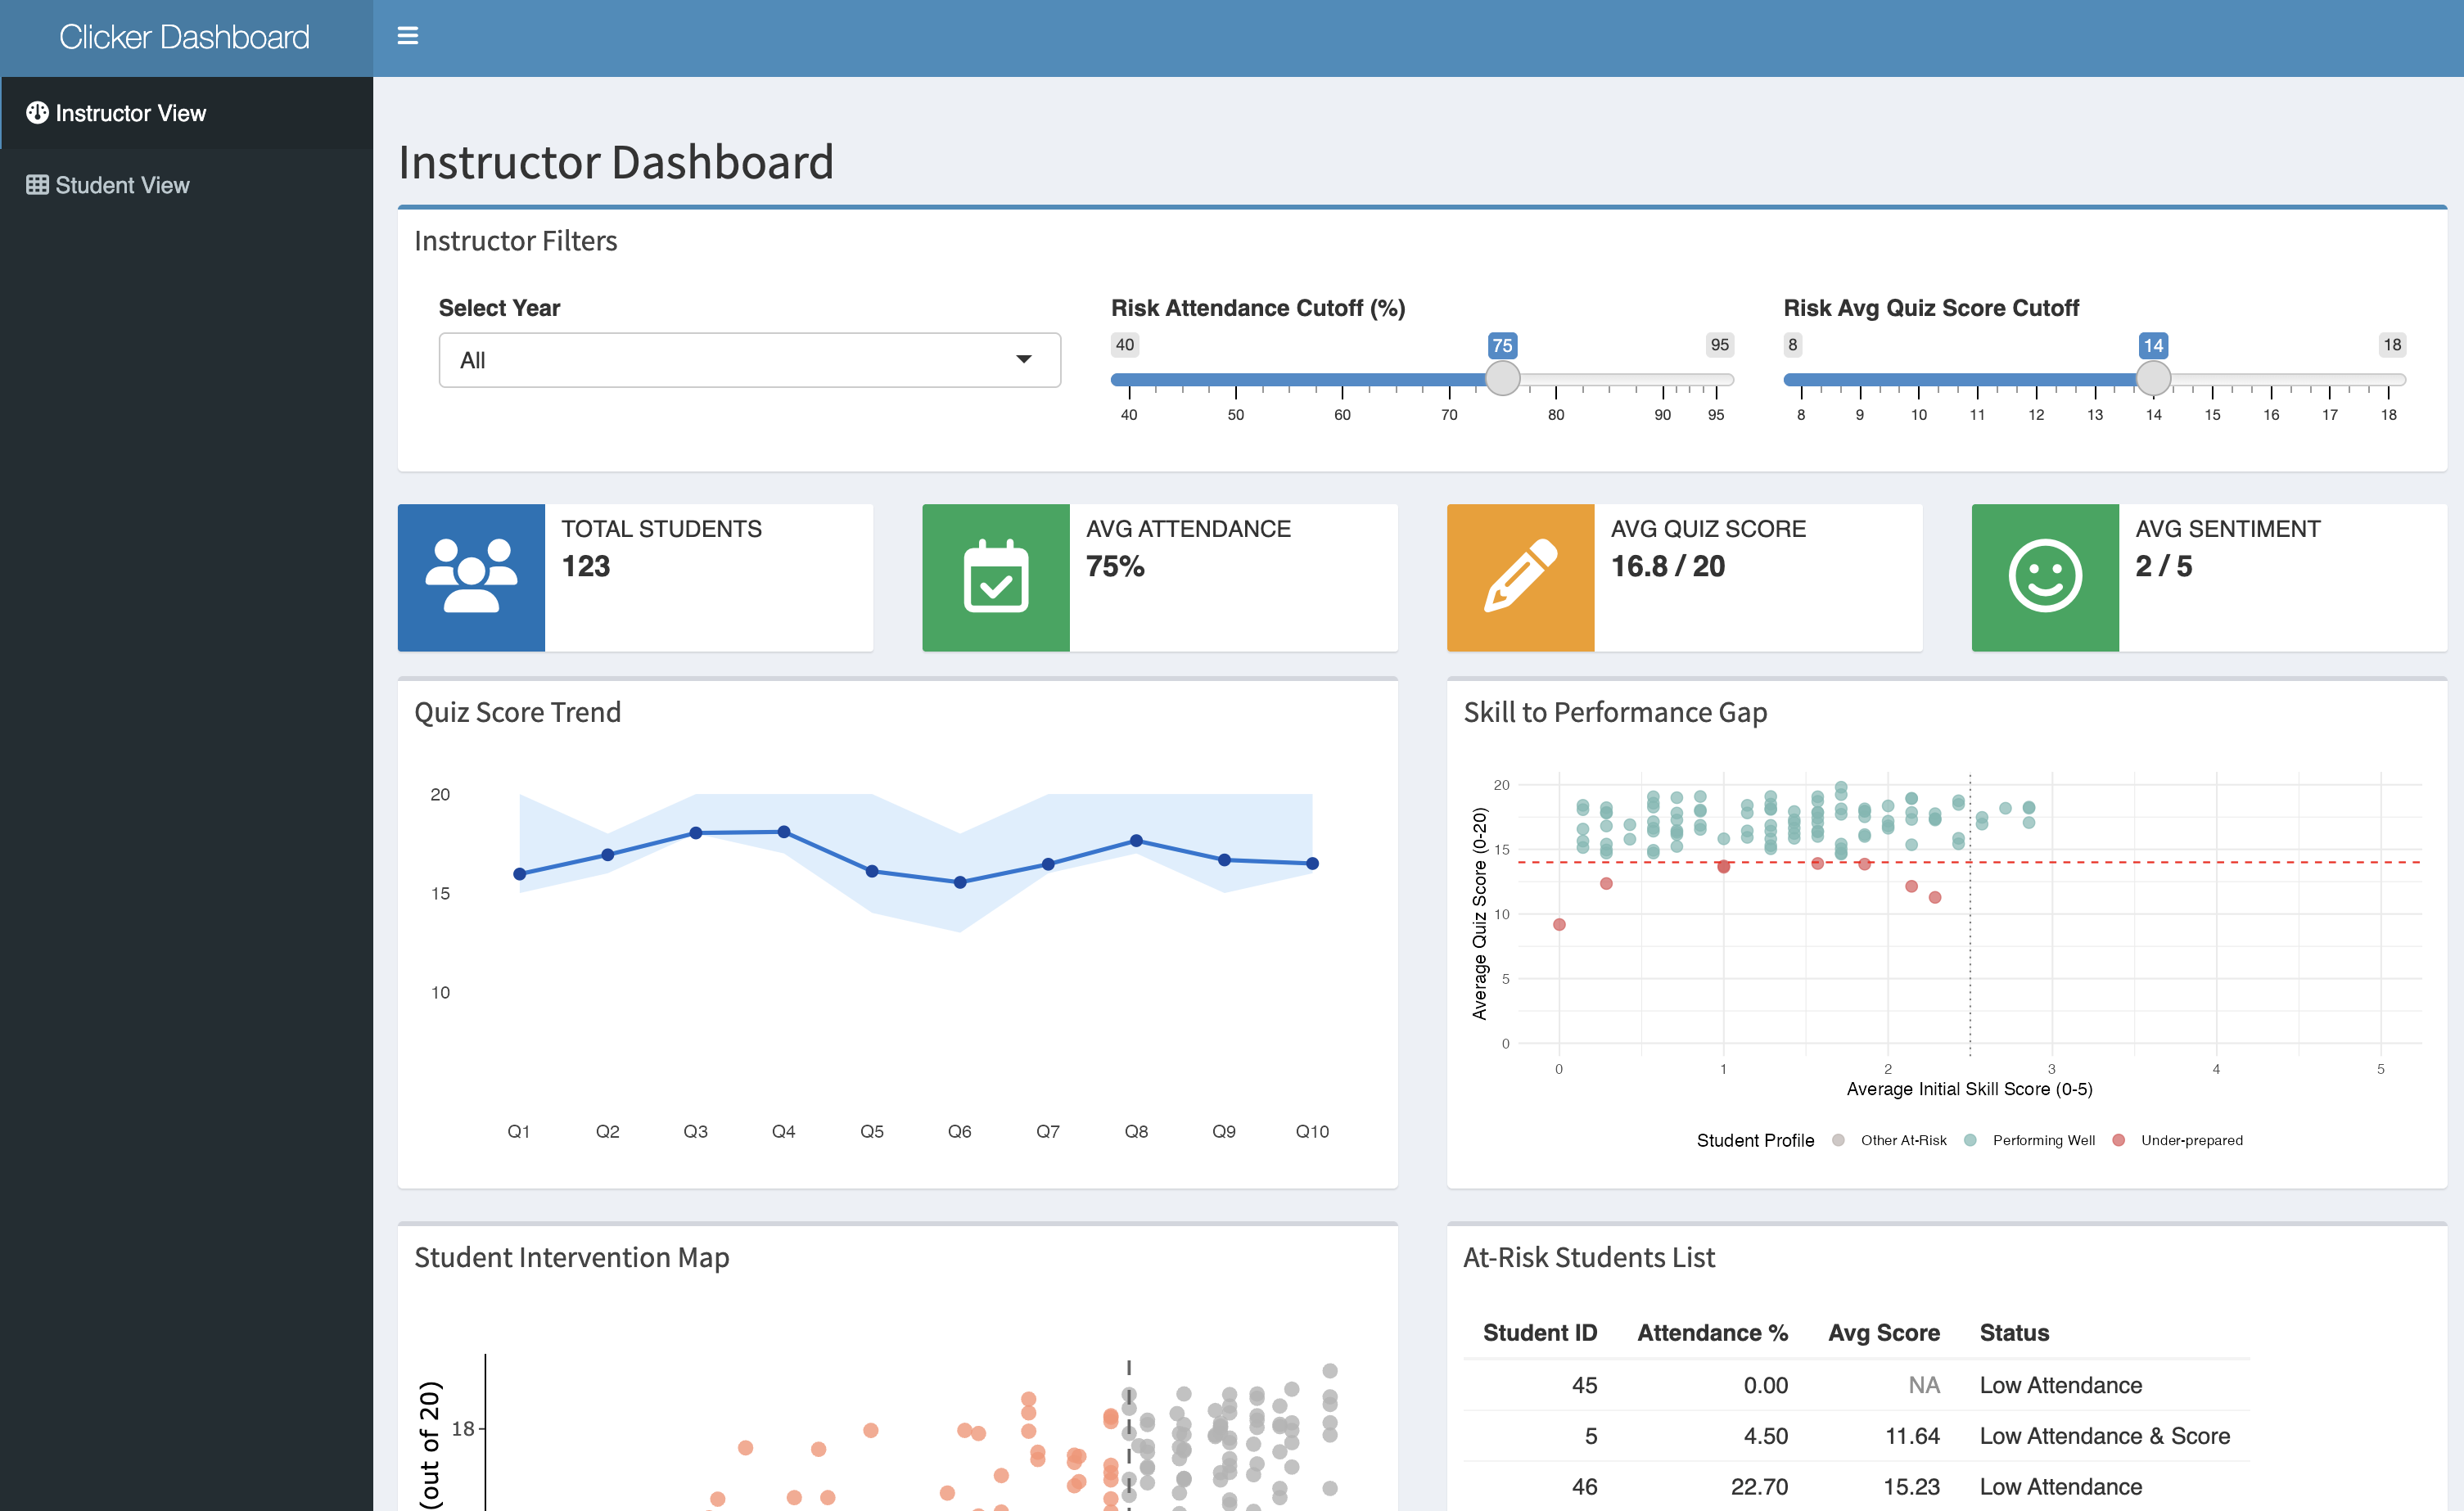
\includegraphics[keepaspectratio]{instructor_dashboard.png}}
\pandocbounded{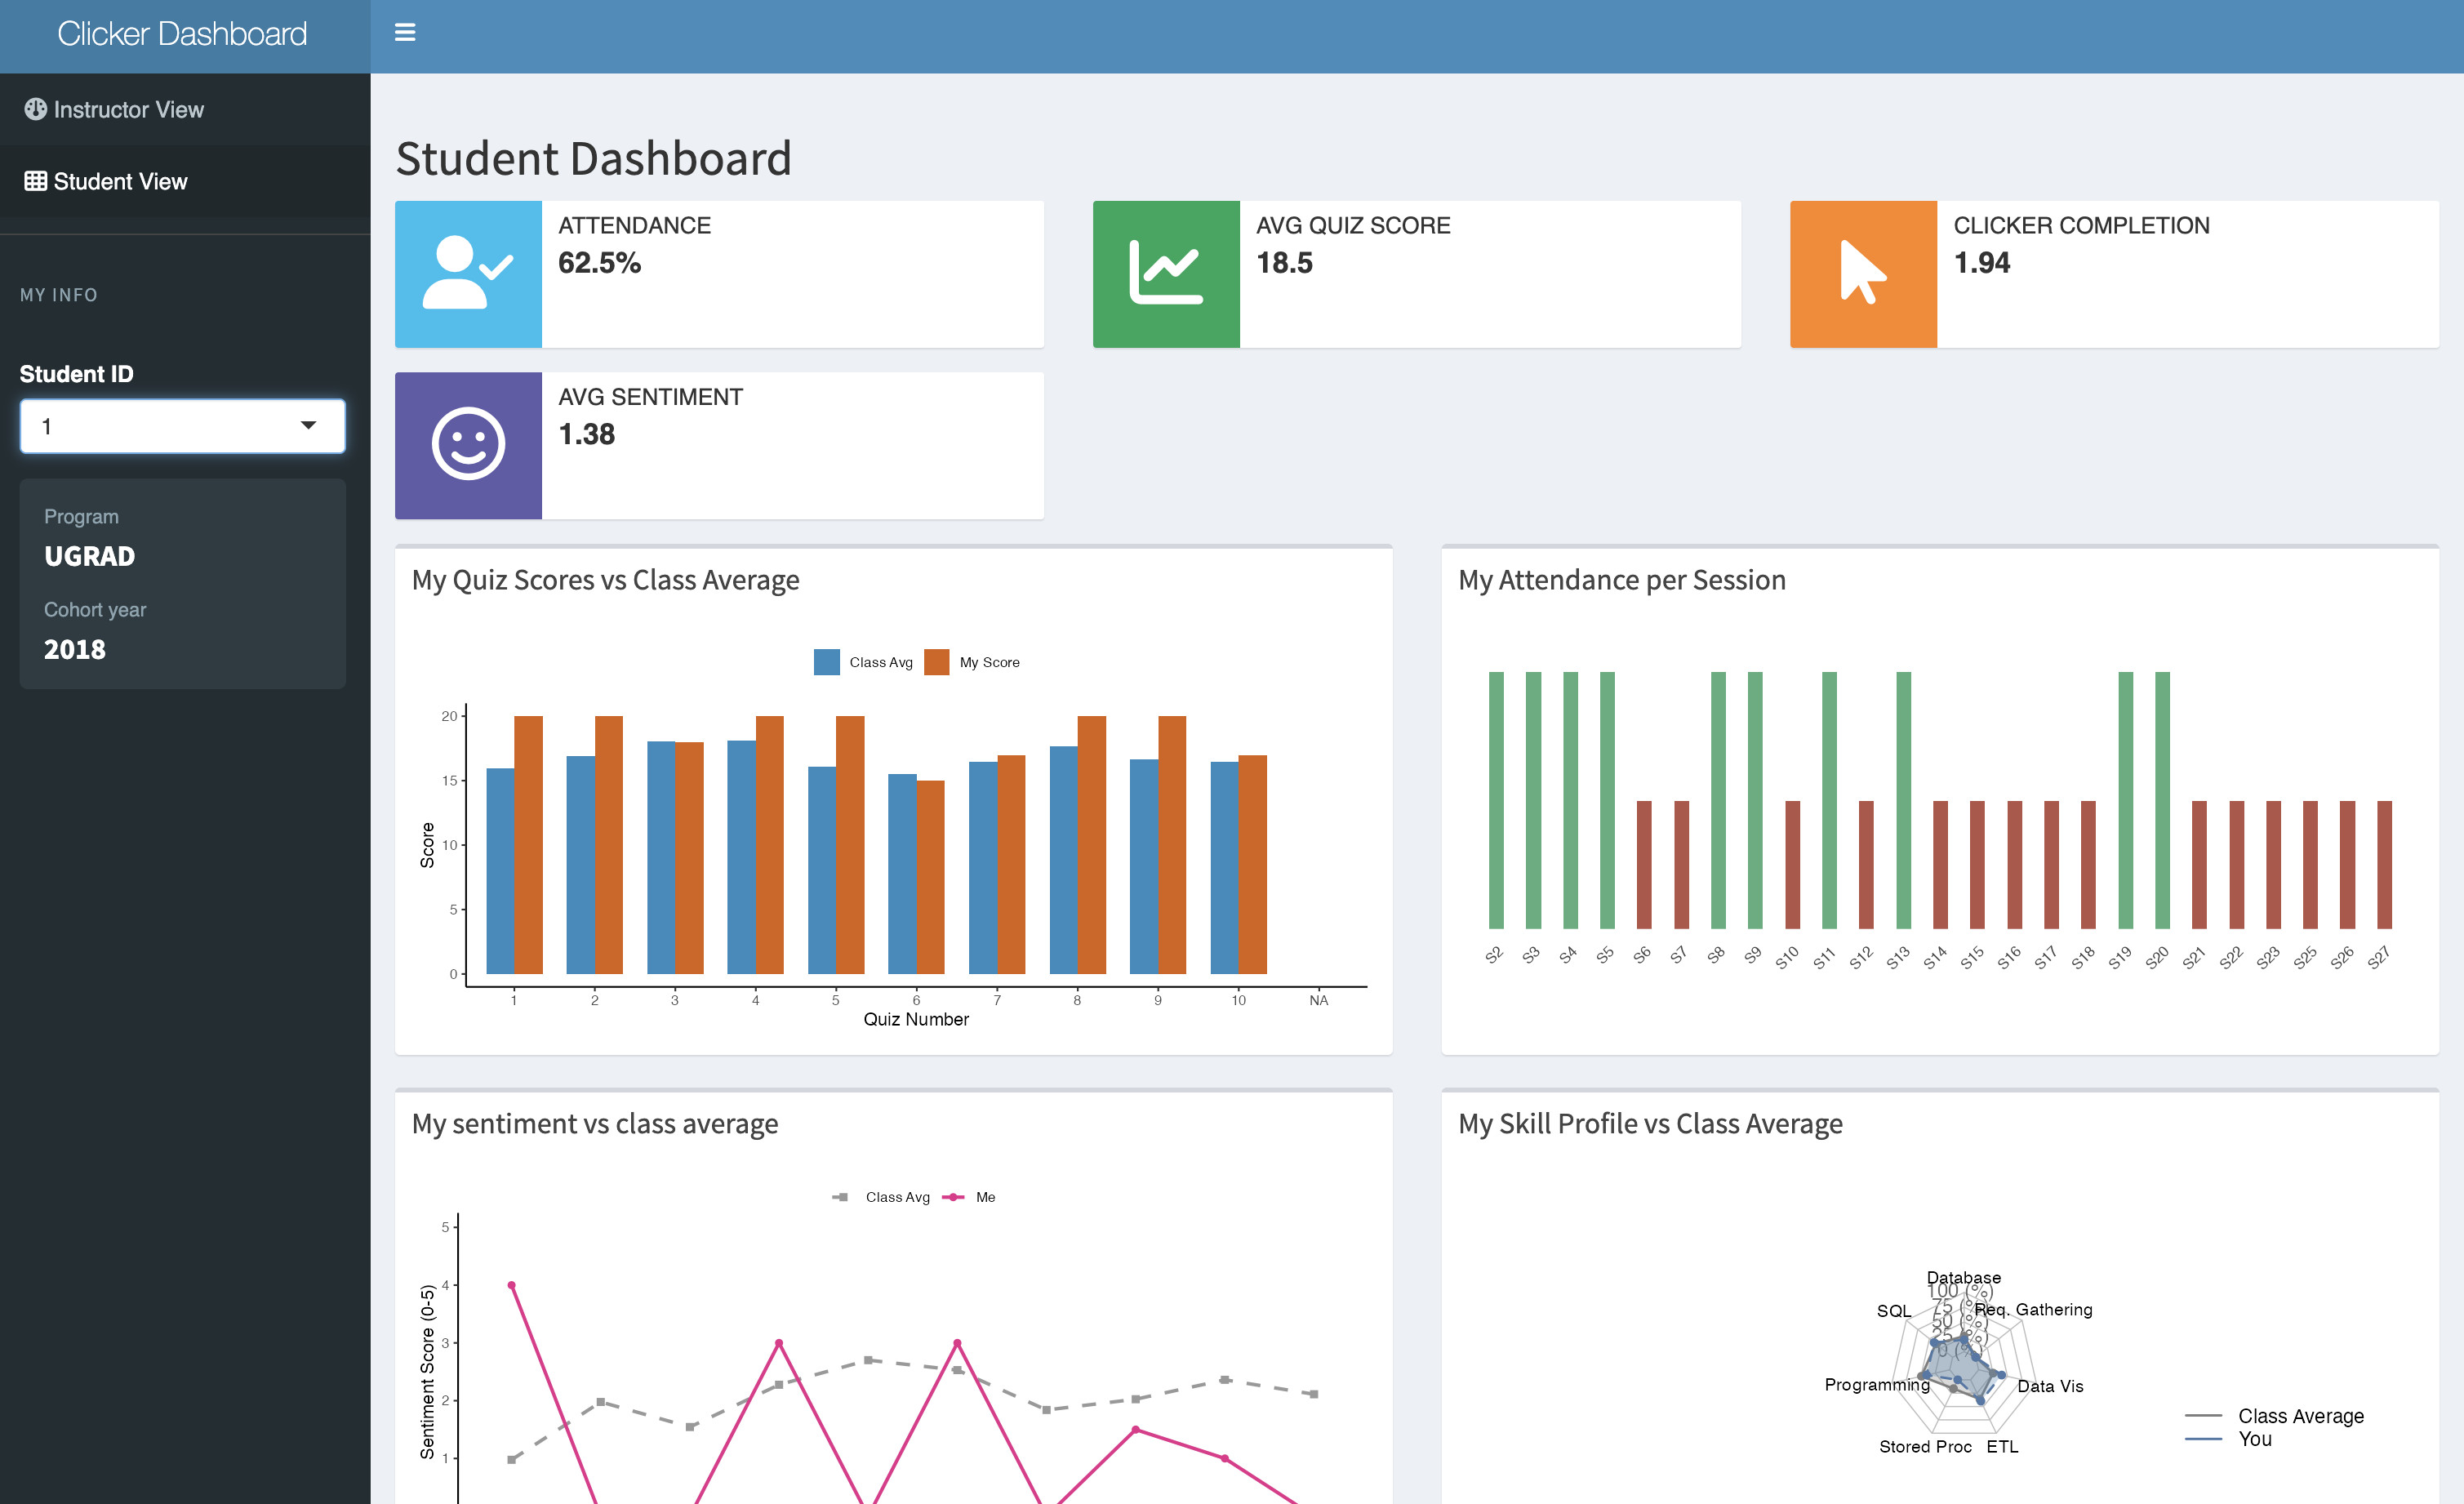
\includegraphics[keepaspectratio]{student_dashboard.png}}

\textbf{Question 6:} Evaluate your group dashboard from the perspective
of the instructor (teacher dashboard) and from the perspective of the
student (student dashboard). What do you like about it, what would you
change or add to it if you had more time?

\emph{Reflection for the student dashboard}

\begin{itemize}
\tightlist
\item
  What do you like about it?

  \begin{itemize}
  \tightlist
  \item
    I really like the highly personalized nature of the visualizations,
    especially how the radar chart and sentiment trend lines allow
    students to instantly see their individual standing compared to
    class-wide benchmarks.
  \end{itemize}
\item
  What would you change or add to it if you had more time?

  \begin{itemize}
  \tightlist
  \item
    If I had more time, I would implement an ``Automated Resource
    Recommender'' that suggests specific review materials based on the
    quiz topics where a student's score falls significantly below the
    class average.
  \end{itemize}
\item
  What was the biggest challenge you faced? How did you address it?

  \begin{itemize}
  \tightlist
  \item
    The primary challenge was ensuring the sidebar student selector
    seamlessly updated all four disparate plots simultaneously; I
    addressed this by centralizing the data filtering into a single
    reactive function to maintain state consistency.
  \end{itemize}
\end{itemize}

\emph{Reflection for the teacher dashboard}

\begin{itemize}
\tightlist
\item
  What do you like about it?

  \begin{itemize}
  \tightlist
  \item
    The ``Skill to Performance Gap'' scatter plot is excellent because
    it helps instructors identify ``at-risk'' students who may have
    overestimated their initial abilities or are struggling despite high
    prior experience.
  \end{itemize}
\item
  What would you change or add to it if you had more time?

  \begin{itemize}
  \tightlist
  \item
    I would add a direct ``Action'' button within the At-Risk Students
    list that allows the teaching team to send pre-formatted
    intervention emails to specific students directly from the dashboard
    interface.
  \end{itemize}
\item
  What was the biggest challenge you faced? How did you address it?

  \begin{itemize}
  \tightlist
  \item
    Balancing high-level class trends with granular student-level
    details was difficult, so we implemented a hierarchical layout using
    info boxes for quick KPIs and scrolling tables for deeper drill-down
    analysis.
  \end{itemize}
\end{itemize}

\section{Estimate time spent}\label{estimate-time-spent}

\textbf{We want to give students an estimate of how much time this
homework will take. Please indicate how many hours you spent to complete
this homework here.}

\begin{itemize}
\tightlist
\item
  We spent 10 hours.
\end{itemize}

\section{Generative AI usage}\label{generative-ai-usage}

\textbf{As stated in the course syllabus, using generative AI is allowed
to help you as you complete this homework. We are interested in how it
is being used and whether it is helpful for you.}

\begin{itemize}
\tightlist
\item
  How much did you use generative AI (e.g., not at all, some, most, or
  all the questions) and which one did you use? =\textgreater{} We used
  generative AI to most of the questions.
\item
  If you used generative AI, how did you use it and was it helpful?
  =\textgreater{} We primarily leveraged AI to write complex code
  structures, debug reactive data flows, and refine the UI styling \#
  Submit Project
\end{itemize}

This is the end of the group project. Please \textbf{Knit to Word} (if
you run into an issue, you can knit to PDF). The resulting file has to
show both the R code and R output. Upload it on Canvas before the due
date.

\end{document}
